\documentclass[12pt, oneside, a4paper]{package}

%%%%%%%%%%%%%%%%%%%%%%%%%%%%%%
%%%%%%%%%%  INFOS   %%%%%%%%%%
%%%%%%%%%%%%%%%%%%%%%%%%%%%%%%
\author{Floriane PICOLO}
\date{08 décembre 2023}
\title{Étude de l'évolution des gènes codant les protéines de transduction des signaux intracellulaires chez les animaux}
\ecoledoctorale{SSBCV}
\equipe{BINGO - Biologie Intégrative des Gonades\\ \small UMR0085 Physiologie de la Reproduction et des Comportements INRAe Centre Val de Loire}
\specialite{Bioinformatique}
\directeur{M}{MONGET Philippe}{Directeur de recherche, Inrae}
\encadrant{M}{PIÉGU Benoît}{Ingénieur de recherche, Inrae}
\president{Mme}{DUITTOZ Anne}{Professeure, Université de Tours}
\rapporteura{M}{BOBE Julien}{Directeur de recherche, Inrae}
\rapporteurb{M}{FARAUT Thomas}{Chargé de recherche, Inrae}
\jurya{Mme}{LANDES Claudine}{Professeure, Université d'Angers}


%%%%%%%%%%%%%%%%%%%%%%%%%%%%%%
%%%%%%%%%%   MAIN   %%%%%%%%%%
%%%%%%%%%%%%%%%%%%%%%%%%%%%%%%
\begin{document}
    \pagedegarde
    \clearpage

    \pagestyle{empty}
    \chapter*{Remerciements}
\thispagestyle{empty}
\onehalfspacing

\par Cette thèse a été réalisée sous la direction de Philippe Monget au sein de l’équipe Biologie INtégrative des GOnades (BINGO) et sous l’encadrement de Benoît Piégu de l’unité Physiologie de la Reproduction et des Comportements (PRC) à l’INRAE de Nouzilly et grâce aux financements de l’Université de Tours. 
\par Je remercie donc l’ensemble des membres de la direction d’unité et tout particulièrement Sophie Mary, Anne Mychak, Ghyslaine Ploux et Sandra Cavalie pour leur aide administrative.
\par Je tiens principalement à remercier les membres du jury d’avoir accepté d’évaluer mon travail, Julien Bobe et Thomas Faraud en tant que rapporteurs ainsi que Anne Duittoz et Claudine Landes en tant qu’examinatrices. 
\par Un profond merci à mon directeur de thèse Philippe Monget pour avoir cru en moi dès le début de mon premier stage en 2016 puis en 2019 et de m’avoir donné cette chance de réaliser une thèse sur un sujet passionnant. Tu as été un réel soutien sur le plan scientifique bien évidemment, pour tous les conseils durant ces trois années, mais surtout pour ton efficacité sans nom dans les retours que ce soit sur les articles ou ce manuscrit. Et tu as également été une bonne épaule pour moi, la doctorante un peu (\textit{beaucoup}) fragile émotionnellement, et qui n’a pas toujours été facile à gérer. Et je tiens également à te dire que je suis ravie que tu ne viennes pas à ma soutenance avec une perruque bleu-blanc-rouge malgré une défaite douloureuse de la France au Rugby. 
\par Je souhaite également remercier mon encadrant Benoît Piégu, pour le soutien et les déblocages sur R. Merci d’avoir insisté si \textbf{lourdement} pour que je sauvegarde mes avancements sur GIT, tu auras finalement eu raison de moi, malgré ma ténacité à te tenir tête. On se souviendra des petites blagues aux JOBIM 2023, mais aussi de toutes celles durant ces trois ans. Et un merci tout particulier pour ces parties de ping-pong mailistique durant la rédaction.
\par Merci à Elis, le chef de notre équipe BINGO. Je n’aurais finalement jamais goûté aux chocolats que tu prétends donner à tous les membres de l’équipe, venant pour tes superbes conseils dignes d’un psychologue. Merci d’être toi, et de m’avoir intégré dans l’équipe.
\par Merci à tous les membres de l’équipe BINGO : Sébastien Elis, Philippe Monget, Marie- Émilie Lebachelier, Sophie Fouchécourt, Virginie Maillard, Peggy Jarrier-Gaillard, Pascal Papillier, Rozenn Dalbies-Tran, Véronique Cadoret, Sandrine Fréret, Ghylène Goudet, Maria-Teresa Pellicer-Rubio, Catherine Taragnat, Svetlana Uzbekova, Laetitia Corset, Cécile Douet, Stéphanie Martinet, Charline Pontlevoy, Claire Vignault, Ophélie Téteau, Alice Desmarchais et Anna Grandchamp.
\par Un merci tout particulier à Sophie Fouchécourt qui a été la première à croire en moi et à me donner cette chance lors d’un stage en DUT en 2016 alors que je n’étais qu’une novice en bio-informatique. Merci de m’avoir accueilli et de m’avoir fait confiance. 
\par Un grand merci également à Michel Laurin et Jérémie Bardin du MNHN de Paris avec qui nous avons grandement collaboré avec un immense plaisir. Bien que l’on ne se soit jamais rencontré, j’ai adoré travailler avec vous. 
\par Un merci à l’équipe de PIXANIM, Valoch, Ana Paula ou AP, Dany, Mimi, Cholet et Jérôme de m’avoir accueillie dans leur bureau pour prendre le café, se raconter nos péripéties, rigoler, faire des compétitions de pédantix et peindre même à l’occasion ! Chaque instant était un plaisir avec vous. 
\par Je remercie aussi les stagiaires de l’équipe Maoui alias le meilleur stagiaire dont je me souviendrais toujours de l’histoire du vélo dans le bus, et tes skills éclatés au sol sur Excel. Et Mapâte la meilleure piou-piou devenue PIOUUU maintenant avec qui on a beaucoup rigolé de ta drôle de passion pour les diverticules, et d’ailleurs, je reste fan de tes slides animés. 
\par Je vais remercier également les zozos du fond du couloir qui font énormément de bruits sans fermer leur porte, les doctorants de l’équipe SENSOR bien évidemment, dont le Bourdz mon partenaire de crêpe et de chouchen, Loïse celle qui a copié ma date de soutenance, je ne serais pas là pour te voir, mais force ! Et entre autres, Mathy que j’ai allégrement embêté en cette fin de thèse.
\par À Marie et Coline, mes co-thésardes préférées, qui m’ont sorti de l’isolement après 1 an de thèse cloitrée à la maison puis dans un bureau isolé au sous-sol. Marie, tu as été d’un soutien immense durant cette thèse. Merci pour tous tes conseils, mais aussi pour toutes ces conversations dans le bureau, et tous ces BeReal ensemble. Oui, c’est Michel, tu donnes pas de nouvelles. Et Coline la meilleure thésarde du monde, un modèle d’exemple d’exemplarité ! Sous tes petits mots fleuris, j’ai su déceler tout l’amour que tu m’apportais, et finalement… bon, je t’aime aussi un peu en retour. Avec toi, c’est l’amour vache (je suis hyper drôle) mais j’ai passé que des bons moments à gueuler avec toi (\textit{et sur toi}). D’ailleurs, je t’offre ma voiture, parce que finalement tu l’as plus conduite que moi, et on sait pourquoi. Finalement, à linera, on ne se fait pas que des collègues, on se fait aussi des bêtes de copines.
\par Un énorme merci aussi à Mimi, la plus fun de ma vie, qui prend si soin de moi. Tu m’auras mise une musique par jour dans la tête, tu m’auras épuisée de ton trop pleins d’énergie et de tous tes uppercuts, mais tu vas me manquer quand tu seras de l’autre côté de l’Atlantique. J’ai adoré te faire des chasses aux trésors et dessiner sur ton bureau pour voir mon bureau multicolore en retour. C’était de bonne guerre. Et un big up à Pouf, Joël et sa poire.
\par Et puis 3 ans, c’est aussi partager son quotidien avec ses voisins ! Merci aux Velpotes : Romain, Pierre, Valentin, Léa et Mathilde. Vous avez rythmé ma vie en partageant des soirées jeux, des pétanques ou des dîners, et vous m’avez même remotivé à courir ! On a vécu des moments improbables ensemble comme l’étrangleur ou Bertrand Desplantes qui ont rempli ma boite à souvenirs. Et un petit mot pour Valentin, mon copain de DUT, merci d’avoir repris contact, merci à nos soirées télés, et de m’avoir fait rencontrer Doriane, cette merveilleuse personne que je vois maintenant plus que toi finalement… Vous êtes au top les velpotes. 
\par J’ai également rencontré de formidables personnes grâce à l’Association des Doctorants de Tours dont j’ai été membre pendant mes 3 années et grâce à qui j’ai rencontré mes copaines de Toursnez Ménage qui m’ont chaleureusement accueilli dans leurs bureaux : Antonin, Yopo, Léa, Thomas, Romain, Igor, Yegor, Guillaume, Théo, Adam, Pierre, Sylvain, Merve, Maxime et Marion ! Que des numéros un dans cette team ! Ça aura été un plaisir de vous gronder chaque jeudi pour que vous veniez faire la fête ! 
\par Dans cette même veine, j’aimerais faire un aparté pour Romain, mon voisin et maintenant meilleur ami, j’ai passé de merveilleux moments avec toi, à rigoler et faire les andouilles (\textit{qu’on adore}). Puis notre trio de l’enfer avec Thomas, à chanter sur les quais de Loire ou juste à se raconter nos vies sur la place Velpeau jusqu’à pas d’heure. Et aussi merci de m’avoir fait rencontrer Sam, notre artiste qui m’a aidé à décompresser pendant la rédaction avec nos jeux de coop. Merci !
\par Et puis je suis obligé de remercier dignement mes parents adoptifs du Shamrock, Annie et Fafa ! Deux formidables personnes, à qui je souhaite un bon départ vers de nouveaux horizons. Annie, merci d’avoir été ma maman à Tours, toujours à nous vouloir nous faire plaisir et à prendre soin de nous. Et que vive longtemps le PICOLO Grande !
\par J’aimerais également remercier du fond de mon cœur, le serveur discord des doctorants « PhD Student » que j’ai rejoint le premier jour de thèse, et que je n’ai jamais lâché depuis. De nombreuses amitiés se sont créées grâce à cette plateforme en ligne, et on a pu se soutenir et rire pendant la pandémie, mais bien plus après notamment à travers les IRL, mais aussi en comptant l’heure (\textit{ça n’a pas de sens}) mais merci aux horlogistes. 
\par Un grand merci à Anana, ma plus belle rencontre sur ce serveur, qui au premier abord n’était qu’une camarade de thèse, mais qui s’est transformé en amitié si intense. Je ne compte plus les allers-retours jusqu’à Lille pour passer un week-end avec toi et les dinos LoloR et Ouistiti. Merci d’être la personne que tu es, tu m’as fait grandir sur bien des sujets et notamment la communication. Finalement, si j’arrive à m’ouvrir dans ses remerciements, c’est peut-être grâce à toi. 
\par Un merci à Galaad aussi, j’ai adoré nos échanges, nos tierlists, et nos jeux (\textit{achetés pour ne plus y toucher}), notre projet de tout plaquer pour lancer une chaîne Twitch n’aura finalement pas eu lieu, mais on avait un si beau concept. Je le garde en tête. Et un gros signe JuL à notre groupe Salut l’Ariège, et à nos AG exceptionnelles pour organiser nos vacances. 
\par Un merci plus général aux équipes de modération du serveur « PhD Student ». En deux ans de modération, j’en ai vu des camarades, et j’ai adoré travailler avec chacun d’entre vous. Un jour, je partirais, mais je suis sûre que mes poulains sauront rédiger des comptes rendus qui me rendront digne (\textit{j’en fais des tonnes}). Courge ! 
\par Et puis, jamais très loin, j’ai les copains du master, on ne s’est pas vu normalement, mais c’était pour profiter encore plus lorsque l’on se retrouvait aux BIGDAY, aux JOBIM ou lors des soutenances de thèses. À ma meilleure amie d'étude supérieur, Manon, qui est maintenant Docteure. Tu es la meilleure ne l’oublie pas. 
\par Je remercierai également mes amies du lycée et principalement Angèle et Laurie, mes deux meilleures amies depuis si longtemps et avec qui on ne s’est jamais lâché. Chaque instant avec vous vaut le dé\textit{Tours} (jeu de mot, parce que je reste l’humour du groupe). J’espère qu’un jour les gars (\textit{et nous}) finiront par grandir et on pourra partir sereinement au ski. Enfin, quoique, ça fait tellement de bons souvenirs. 
\par Et enfin ma famille, je ne sais si je trouverai les mots pour vous remercier. À mon père et ma belle-mère qui m’ont toujours écouté me plaindre sans forcément comprendre. À ma maman parfaite et Sergio qui pensent encore que je vais bientôt devenir Avocate, désolée c'est toujours pas ça. À mon frère à qui je souhaite de réussir, tu as des mains en or ma breur. À mon arrière-grand-mère décédée, et à mon arrière-grand-père qui nous a également quitté durant ma rédaction. À mon grand-père et à ma merveilleuse grand-mère. Ça n’a jamais été facile de se dire je t’aime, mais je crois que je peux au moins l’écrire. \textbf{Je vous aime.} 
\par Et puis un petit merci, à mon chat, Nuggets. Ce gros sac à prout a rythmé mes nuits et mes insomnies. Un enfant capricieux, mais que l’on aime de tout son cœur. 
\par Alors voilà que s’achève 3 années de ma vie. Quand je repense à Philippe le 15 novembre 2020 me disant « tu verras, 36 mois ça passe très vite » et moi lui riant au nez, finalement, tu avais raison. En 36 mois, j’ai eu trois covids compliqués, dont un durant ma soutenance, une grippe, un accident de voiture, et je suis aussi passée sous une voiture. J’ai eu le feu dans mon appartement et deux dégâts des eaux. Je me suis fait voler mes affaires sur les bords de Loire et j’ai eu un étrangleur dans mon immeuble. Mais j’ai également j’ai fait partie de deux associations incroyables, créé un jeu de piste sur la ville de Lyon et créé un cocktail au Shamrock de Tours, organisé deux IRL géantes pour les doctorant.es en France, couru 10 km et battu mon propre record. 
\par\textbf{\textit{Mais surtout, j’ai réussi à écrire cette thèse.}}  

% \pagestyle{empty}
% \AddToShipoutPictureBG*{%
%   \AtPageLowerLeft{%
%     \includegraphics[width=0.2\paperwidth,height=0.2\paperheight]{figures/logos/nugg.png}%
%   }%
% }

\begin{flushright}
Merci à vous.\\
Bravo à moi.
\end{flushright}
% \pagestyle{empty}
\newpage
    \tableofcontents\thispagestyle{empty}         % table des matières principale
    \listoffigures\thispagestyle{empty}
    
    \pagestyle{plain}
    \chapter[Introduction]{Introduction}
\thispagestyle{firstpage}
\onehalfspacing
\setcounter{page}{1}
%%% NOUVELLE SECTION
\par Si l’évolution peut avoir plusieurs définitions dans le dictionnaire, elle a une définition très spécifique dans l’univers de la biologie. En effet, l'évolution se réfère à la modification progressive du monde vivant au fil du temps. L’évolution est un mécanisme complexe et permet la diversité de la vie sur Terre. Elle peut se caractériser par plusieurs sous-notions comme la notion d’hérédité, d’adaptation, de sélection, de coévolution, de mutation ou encore de spéciation. Ces grandes notions vont être importantes pour la suite de l’introduction : la génétique, l’étude des gènes, et génomique, celle des génomes. Dans les prochains chapitres introductifs, nous détaillerons ce que sont les gènes et génomes, la diversité animale, et brièvement la communication cellulaire. 

%%% GENES ET GENOMES
\section{Gènes et génomes}\label{genes}
\par Les gènes sont des fragments d’ADN (acide désoxyribonucléique) qui comportent l’information génétique de chaque organisme vivant. L’ADN mitochondrial est stocké principalement au niveau du noyau de la cellule pour les organismes eucaryotes (à la différence des organismes procaryotes, donc sans noyau où l’ADN est retrouvé concentré en région que l’on appelle le nucléoïde). Les gènes sont transmis d’une génération à une autre, mais sont soumis à des modifications aussi appelées « mutations » de leur séquence nucléotidique (succession d’éléments : adénine (A), cytosine (C), guanine (G) et thymine (T)). Pour être traduit en protéine, la séquence nucléotidique d’un gène se lit par codon, une suite de 3 nucléotides. Chaque combinaison de codon correspond à un acide aminé. Il existe 20 acides aminés communs à l’ensemble du vivant \parencite{ambrogelly_natural_2007}. Une suite d’acides aminés commençant par un codon initiateur et se finissant par un codon terminal deviendra sera dans un premier temps transcrit en ARNm (acide ribonucléique messager) puis traduit en protéine par le biais de la traduction réalisée par un ribosome.
\par La transcription a lieu dans le noyau de la cellule, et transcrit donc la séquence nucléotidique en séquence complémentaire. Il est important de préciser qu’un même gène peut conduire à une multitude de protéines \parencite{breathnach_organization_1981}. En effet, les gènes sont constitués de sous-parties : d’un promoteur (partie initiatrice de la transcription), d’exons (parties codantes de l’ADN, elles vont aider à déterminer la structure de la protéine) et d’introns (parties non codantes de l’ADN, elles vont jouer un rôle dans la régulation de l’expression génique) \parencite{keren_alternative_2010, shaul_how_2017}. Chez les eucaryotes, avant que l’ARNm ne soit traduit en protéines, il va être édité et ce phénomène s’appelle la maturation. Les introns vont être épissés, et les exons conservés. Un même gène peut avoir différentes combinaisons d’exons assemblés, ce qui peut conduire à avoir plusieurs protéines différentes (Figure \ref{fig:1_genetoprotein}).
\par Comme on a pu le voir, les gènes sont des petits éléments complexes, mais indispensables à un organisme. L’ensemble des gènes constitue le génome. 

\begin{figure}[H]
    \centering
    \includegraphics[width=1\textwidth]{figures/corps/figure1.png}
    \caption{Schéma d'un gène à une protéine}
    \label{fig:1_genetoprotein}
\end{figure}
Légende : Les différentes étapes d’un gène à une protéine sont représentées à l’exception de la maturation (épissage alternatif).\\

%%% EVOLUTION DES GENES, MUTATION DELETIONS INSERTIONS
\subsection{Évolution des gènes : mutations, délétions, insertions}\label{mutations}
\par L'ADN peut subir des changements de différentes manières. Tout d'abord, il y a les mutations, qui peuvent être spontanées, se produisant lors de la transmission de l'information génétique à la descendance, ou environnementales, résultant d'altérations dues à des facteurs extérieurs tels que les virus et le soleil, entre autres. Ces mutations affectent la séquence de nucléotides et peuvent entraîner des conséquences plus ou moins graves en fonction de leur nature.
\par Une mutation peut être une substitution d’un nucléotide par un autre. En fonction du nucléotide touché, elle peut avoir plus ou moins de conséquences. Le code génétique est doté de quelques redondances concernant la traduction des acides aminés. Par exemple, la sérine est un acide aminé codé par 6 codons différents (UCU, UCC, UCA, UCG, AGU et AGC). Si la séquence est initialement UCG, et que la substitution a lieu sur le 3ème nucléotide de la séquence : il n’y aura pas d’impact sur la traduction du codon, quelle que soit la substitution. Cette mutation est dite silencieuse. Si la substitution a lieu sur le 2ème nucléotide, de telle façon à former UAG, on obtient donc un codon stop, ce qui veut dire que le ribosome n'ira pas au-delà lors de la traduction. La protéine ne sera donc pas celle initialement prévue, possiblement tronquée et non fonctionnelle. Cette mutation est dite non-sens. Et enfin si la substitution a lieu sur le 1ème nucléotide, de telle façon à former GCC, on obtient un nouvel acide aminé qui est l'alanine. Cette mutation est dite faux sens car la protéine finale sera impactée par ce changement d'acide aminé (Figure \ref{fig:2_mutations}).
\par Une mutation peut aussi prendre la forme d'une insertion ou d'une délétion, c'est-à-dire l'ajout ou la suppression d'un nucléotide dans la séquence d'ADN. Étant donné que la séquence se lit en codons, cela perturbera le "cadre de lecture" si un ou plusieurs nucléotides (non multiple de 3) sont ajoutés ou supprimés. Le cadre de lecture détermine comment les codons seront lus par le ribosome lors de la traduction (Figure \ref{fig:2_mutations}). 
\par Il existe également la recombinaison génique qui est un déplacement d’une région d’ADN vers une autre. Lors de ces recombinaisons, il se peut que la séquence soit également dupliquée \parencite{sasaki_genome_2010, stewart_homologous_2022, syeda_recombination_2014}. Des copies de gènes ou des copies de séquence sont alors ajoutées dans la séquence, que l’on appelle des duplications segmentales. Lorsqu’il s’agit de gène entièrement dupliqué, différents scénarios peuvent avoir lieu. Le gène dupliqué peut garder la fonction initiale du gène original. Le gène peut acquérir une nouvelle fonction proche, voire une spécialisation (spatio-temporel) au gène original. Mais il peut également se pseudogéniser, c’est-à-dire devenir non fonctionnel par une altération de sa séquence. 
\par Les mutations ont donc un effet direct sur la séquence nucléotidique, mais également sur la protéine et la fonctionnalité de celle-ci, effet qui peut être avantageux ou désavantageux \parencite{long_origin_2003}. Les duplications sont également un moteur de l’évolution. L’exemple de la famille des globines peut en attester \parencite{weatherall_molecular_1976}. En effet, les duplications des globines ont permis aux vertébrés de s’adapter à différents environnements ou à des contraintes physiologiques. 
\par Les duplications segmentales sont des événements à échelle restreinte, mais il existe également une autre forme de duplication, la duplication complète du génome.


%%% DUPLICATION COMPLETE DE GENOME
\subsection{Duplication complète de génome}\label{wgd}
\par La duplication de génome (Whole Génome Duplication en anglais, WGD) est un événement de polyploïdisation, c’est-à-dire une duplication du nombre de chromosomes. La polyploïdisation est très courante dans le règne des plantes, puisque environ 70\% des angiospermes ont eu au moins un événement de polyploïdisation \parencite{masterson_stomatal_1994, soltis_polyploidy_2009}.
\par Les premières études démontrant des phénomènes de duplication ancestrale de génome chez les plantes date des années 2000 chez \textit{Arabidopsis Thaliana} \parencite{blanc_recent_2003, bowers_unravelling_2003, the_arabidopsis_genome_initiative_analysis_2000} et concernant le règne des animaux, les duplications de génome sont mises en évidence chez les vertébrés à partir de 1994 \parencite{holland_gene_1994, nakatani_reconstruction_2007}. Le groupe des vertébrés est notamment marqué par la succession de deux duplications complètes de génome par rapport aux invertébrés \parencite{dehal_two_2005}. Ce double événement est d’ailleurs probablement impliqué dans la divergence des espèces de vertébrés. Le groupe des vertébrés ne comptant « que » 72 000 espèces (contre environ 1 000 000 d’invertébrés d’après la Classification phylogénétique du Vivant \parencite{lecointre_classification_2016}) regroupe, pour autant, une multitude d’espèces de tailles et de morphologies, d’environnements ou de modes de reproduction complètement différentes.
\par D’autres groupes ont également vécu des duplications de génome supplémentaires, comme le groupe des poissons téléostéens \parencite{braasch_polyploidy_2012, meyer_2r_2005}, dont celui des salmonidés et des carpes \parencite{lien_atlantic_2016, xu_allotetraploid_2019} que nous verrons par la suite plus en détail (Chapitre  ~\ref{teleost} page ~\pageref{teleost}). 
\par Une famille de gènes a notamment permis de mettre en lumière les duplications de génomes : la famille des Hox (venant de « \textit{homeobox} »). Les gènes Hox sont des facteurs de transcription présents chez la quasi-totalité des bilatériens (\textit{Bilateria}). Leur organisation génomique est relativement complexe, c’est-à-dire localisés par bloc de plusieurs gènes à la suite. Par exemple, la drosophile compte 8 gènes en 2 complexes, et l’homme 39 gènes organisés en 4 complexes, chacun est subdivisé en 13 paralogues (gènes Hox1 jusqu’à Hox13) \parencite{hoegg_hox_2005, meyer_vertebrate_1999, rux_hox_2017}. Chez les téléostéens, on compte pas moins de 63 gènes Hox \parencite{meyer_vertebrate_1999, stellwag_hox_1999} (Figure \ref{fig:3_hox}). De ces premières découvertes, il a été question de trouver l’origine de ces multiples duplications, et de déterminer s’il s’agissait de duplications segmentales ou de duplications de génome. 

\begin{figure}[H]
    \centering
    \includegraphics[width=0.85\textwidth]{figures/corps/figure2.png}
    \caption{Différents types de mutations}
    \label{fig:2_mutations}
\end{figure}
Légende : Représentation des mutations silencieuses, faux sens, non-sens, des insertions et délétion à partir d’une même séquence initiale. \newpage


\par Ces duplications de génomes sont également étudiées pour la recherche médicale. Il a récemment été montré que dans plusieurs cas de tumeurs, des duplications de génome étaient impliquées \parencite{gemble_genetic_2022}. Cette étude montre une forte instabilité génétique après des événements de WGD, ce qui favoriserait les multiples mutations. 
Les duplications de génome sont également connues pour être suivies de perte massive de gènes dupliqués \parencite{inoue_rapid_2015, jaillon_genome_2004}. Ce phénomène, a pour conséquence la rediploïdisation et consiste en un retour au nombre initial de gènes et non des chromosomes. Pour certains gènes, une seule copie des gènes sera maintenue, ce qui réduit grandement le nombre de paralogues issus de duplication de génome complet \parencite{byrne_yeast_2005}. Par exemple, si le génome de la drosophile partage un patrimoine génétique en commun avec l’homme et compte environ 15 000 gènes codant des protéines, et avec les 2 duplications de génome qu’ont vécu les vertébrés, l’homme devrait avoir environ 60 000 gènes, or, il n’en compte qu’environ 22 000 gènes codants des protéines. Par ailleurs, certains gènes maintenus en duplicat sont responsables de démence chez l’homme, comme la duplication du gène SNCA impliqué dans la maladie de Parkinson \parencite{chartier-harlin_alpha-synuclein_2004, ibanez_causal_2004}. 
La question que nous pouvons nous poser est : quelle force évolutive régit les gènes restés en duplicat ou revenus en singleton ? 

\subsection{Coévolution}\label{coevo}
\par Concernant la force évolutive qui agit sur les gènes, nous n’avons pas de réponse claire et universelle à donner. Cependant, des pistes pourraient expliquer cette pression, comme celle de la coévolution. La coévolution est le fait que des gènes évoluent ensemble en réponse les uns aux autres \parencite{lovell_integrated_2010}. Et c'est ce que Thompson avait défini en 1994 comme étant la coévolution réciproque \parencite{thompson_coevolutionary_1994}. 
\par Un exemple assez parlant est celui des gènes du système immunitaire. Les gènes du système immunitaire n’ont pas d’autres choix que d’évoluer en fonction de l’évolution des pathogènes qui eux-mêmes évoluent en fonction du système immunitaire \parencite{schlesinger_coevolutionary_2014}. 
\par La coévolution est également très étudiée pour les interactions ligands récepteurs, en effet cette interaction est soumise à une certaine pression notamment au niveau de leur site de liaison qui peut être unique en fonction de la spécificité de la relation. Pour le couple OXT-OXTR (l’ocytocine et son récepteur) par exemple, les séquences moléculaires ont longtemps été pensées comme intactes chez les mammifères, seulement, il a été montré quelques différences subtiles qui seraient corrélées avec les changements comportementaux sexuels chez les primates étudiés \parencite{vargas-pinilla_evolutionary_2015}.

\begin{figure}[H]
    \centering
    \includegraphics[width=1\textwidth]{figures/corps/figure3.png}
    \caption{Organisation des gènes Hox chez la drosophile,\\ les mammifères et les téléostéens}
    \label{fig:3_hox}
\end{figure}
Légende : Chaque carré représente un gène Hox. Pour la drosophile, les clusters vont de 1 à 6 puis de 7 à 13. Pour les mammifères et les téléostéens, ce seront préférentiellement les différentes lettres A à D. Les gènes partageant la même couleur sont des orthologues. 
Entre la drosophile et les mammifères, le gène 2 s’est subdivisé en 2 et 3, et le gène 9 s’est subdivisé en 9 à 13. Les mammifères qui sont un groupe d’espèces à 2 WGD (duplication de génome complet) comptent environ 39 gènes, et les téléostéens (3 WGD) comptent environ 63 gènes Hox. (Par ailleurs, le cluster Dd des téléostéens n’est pas largement représenté par l’ensemble des téléostéens). Cette figure a été réalisée à partir de plusieurs références \cite{amores_zebrafish_1998, guo_hox_2010, lappin_hox_2006, rux_hox_2017}.



\subsection{Naissance et mort des gènes}\label{naissance}
\par Entre les mutations ponctuelles, les duplications de génome, et les pertes massives qui ont suivi, il est question de la naissance et de la mort des gènes. La revue de \cite{kaessmann_origins_2010} détaille les différents types de naissance d’un gène. Nous allons en expliquer quelques-uns. 
\par Dans un premier temps, un nouveau variant d’un gène peut naître d’une mutation ponctuelle. En effet, une mutation peut modifier la séquence nucléotidique d’un gène déjà existant sans qu’il soit pseudogénisé. Un nouveau gène peut apparaître et potentiellement une nouvelle protéine fonctionnelle. 
\par Dans un deuxième temps, la duplication est un moteur clé de la création de nouveaux gènes, que la duplication soit une duplication complète du génome, d’un chromosome uniquement ou même juste localement d’un gène ou d’une partie de séquence. 
\par La naissance des gènes est un mécanisme indispensable à la spéciation et l’adaptation des espèces. Par ailleurs, ce sont des processus très longs, tout comme la mort d’un gène. Si un gène peut naître d’une duplication ou d’une mutation, ce sont les mêmes processus qui peuvent l’amener à la mort. Comme nous l’avons vu dans le Chapitre ~\ref{wgd} page ~\pageref{wgd}, une mutation impliquant un codon stop prématuré peut aboutir à un pseudogène. 
\par Nous pouvons déterminer si un gène est mort en comparant sa séquence à celle d’une autre espèce proche, mais pour laquelle le gène est fonctionnel. À partir de l’alignement de séquence, il est possible de retrouver, comme dans le cas de figure présenté en Figure \ref{fig:4_blast}, une mutation qui remplace un acide aminé par un codon stop (*) par exemple. \newpage

\begin{figure}[H]
    \centering
    \includegraphics[width=1\textwidth]{figures/corps/figure4.png}
    \caption{Exemple d'un pseudogène avec BLAST}
    \label{fig:4_blast}
\end{figure}
Légende : Dans la première partie de la figure, il s’agit d’une capture d’écran de l’alignement des gènes (synténie, décrit en chapitre \ref{genomicus}), centré sur le gène en vert (ENSAOCG00000009653, BCL2) qui est présent chez les espèces \textit{Clown anemonfish} et \textit{Spiny chromis}, mais absent chez \textit{Orange clownfish}. Il y a donc une suspicion de pseudogène, car la séquence semble être conservée pour les gènes à proximité. Une fois la séquence protéique du gène bcl2 de l’espèce \textit{Clown anemonfish} récupérée, on l’aligne sur son génome. Aucune particularité à observer. Puis, on l’aligne sur l’espèce \textit{Orange clownfish}, et là, on remarque qu’il y a un codon stop (*) qui s’est glissé dans la séquence au niveau de l’Arginine. Le gène est bien pseudogénisé chez cette espèce. 

\newpage
\section{Phylogénie des animaux}\label{phylo}
\par La phylogénie s’est définie graduellement. D’abord avec le Suédois Carl Von Linné au XVIII$\textsuperscript{e}$ siècle qui s’impose avec l’idée de biodiversité et sa classification de plus de 10 000 espèces en binôme genre-espèce. Ce sont ensuite les travaux de Lamark au XIX$\textsuperscript{e}$ siècle qui évoquent les liens de parenté et la transmission du patrimoine génétique d’un parent à ses descendants. Et c’est en 1859 que Charles Darwin publie son ouvrage « De l’origine des espèces » qui soudera la théorie de l’évolution selon laquelle les êtres vivants sont issus d’ancêtres communs, et l’évolution des espèces se produit grâce à la sélection naturelle (caractère héréditaire favorisant la reproduction et la survie de l’espèce). 
\par Avec le temps, les méthodes se sont vues améliorées, nous sommes passés d’une classification morphologique à une classification par la séquence ADN. 


\subsection{Principe de la phylogénie}\label{principephylo}
\par Le principe de phylogénie reprend notamment les travaux de Charles Darwin, et repose principalement sur le fait que chaque organisme descend d’un ancêtre commun. On représente communément les relations de parenté entre les organismes dans un arbre. Les arbres sont constitués de branches qui représentent les liens de parentés, et les nœuds les points de divergence. Ils sont construits à partir d’alignement de séquences et permettent de refléter la proximité entre celles-ci. 
\par Différentes méthodes existent afin de parvenir à représenter l’histoire évolutive des séquences : 
\begin{itemize}
    \item Méthode de parcimonie (la méthode la plus simple, car on considère le minimum d’événement évolutif), 
    \item Méthode de distance (on considère la distance entre les espèces par le nombre de différences entre les séquences), 
    \item Méthode basée sur le maximum de vraisemblance (méthode qui va utiliser les probabilités d’obtention d’un arbre en fonction de plusieurs scénarios), 
    \item ou encore des méthodes plus complexes pour des arbres comportant des hybridations et donc ne peut être définie de manière arborescente \parencite{tagu_bio-informatique_2010}.
\end{itemize}
\par Chaque méthode de reconstruction d’arbre a ses avantages et ses faiblesses, et dépend principalement des données et des objectifs. Cependant, il est préférable de combiner plusieurs méthodes et d’utiliser une méthode d’estimation de la robustesse des nœuds une fois l’arbre généré. La robustesse est estimée par la méthode de \textit{bootstrap} par exemple qui consiste à compter le nombre de fois qu’une branche est présente dans un pool d’arbres échantillons obtenu à partir d’alignements prit aléatoirement dans notre jeu de données.
\par Deux types d’études peuvent être considérés en phylogénie. Dans un premier temps, il y a la phylogénie des espèces, qui place des espèces par rapport à d’autres. Et dans un deuxième temps, il y a la phylogénie des gènes qui permet de mettre en relation des similitudes des gènes. Les arbres de gènes peuvent être différents des arbres des espèces. Pour exemple, le gène FOXP2, aussi appelé le « gène de la parole » est présent chez des espèces vertébrées comme l’homme, la souris, la chauve-souris ou encore des oiseaux \parencite{enard_molecular_2002, scharff_evolutionary_2005, webb_foxp2_2005, white_singing_2006}. La séquence protéique est fortement conservée chez toutes les espèces, à l’exception de la chauve-souris qui pourrait être liée à l’écholocalisation chez celle-ci \parencite{li_accelerated_2007}. En représentant l’arbre du gène FOXP2 et l’arbre des espèces, on se rend compte qu’ils ne sont pas identiques ou congruents (Figure \ref{fig:5_foxp2}). 
\par Dans notre cas, nous avons travaillé avec des arbres phylogénétiques de gènes et certains concepts et termes sont à définir, comme l’homologie, l’orthologie et la paralogie.

\begin{figure}[H]
    \centering
    \includegraphics[width=1\textwidth]{figures/corps/figure5.png}
    \caption{Différences entre arbre de gènes et d'espèces}
    \label{fig:5_foxp2}
\end{figure}
Légende : À gauche, il y a l’arbre du gène FOXP2 en fonction de l’alignement des différentes séquences. À droite, il y a l’arbre des espèces. \newpage

\subsection{Homologie, orthologie et paralogie}\label{homologie}
\par Homologie, orthologie et paralogie désignent tous les 3 des degrés différents d’évolution de parcours des gènes. 
\par Le terme homologie se réfère aux similitudes de séquences entre plusieurs gènes, il englobe les termes paralogie et orthologie. Deux gènes ayant un ancêtre commun sont dits « homologues ».
\par La paralogie fait référence à des gènes issus d’une même descendance, mais ayant subi des duplications génétiques au sein d’une même espèce. Ils peuvent avoir subi également des mutations qui ne les rendent pas identiques. De plus, les gènes paralogues n’ont pas forcément la même fonction, il est même plutôt fréquent d’avoir une néo-fonctionnalisation (nouvelle fonction du gène), une sous-fonctionnalisation (les deux gènes acquièrent une sous-fonction de la fonction mère du gène), une spécialisation spatio-temporelle ou une spécialisation de fonction \parencite{kuzmin_retention_2022, force_preservation_1999}.
\par L’orthologie concerne les gènes partageant un ancêtre commun suivi d’un événement de spéciation, donc d’espèces différentes \parencite{fitch_distinguishing_1970}. La définition d’un orthologue est simple lorsqu’on parle de deux gènes, mais se complique rapidement lorsqu’on parle de plusieurs gènes pour plusieurs espèces. Et pourtant, c’est bien grâce aux relations d’orthologie que l’on a fait des avancées en génomique comparative et pour l’annotation des nouveaux génomes séquencés \parencite{huerta-cepas_fast_2017}. 
\par Les relations d’homologies sont donc étroitement liées les unes avec les autres et peuvent être complexes. Au sein des arbres phylogénétiques, il y a à la fois, les orthologues et les paralogues. Pour être plus précis, lorsque des orthologues n’ont pas subi de duplication par la suite, ils sont appelés orthologues directs. Le terme paralogue direct existe également pour les gènes dupliqués au sein d’une même espèce. (Figure \ref{fig:6_ortho}). 
\par Les gènes paralogues issus de duplication de génome sont appelés onhologue en mémoire à Ohno qui a mis en lumière les duplications de génome chez les vertébrés \parencite{ohno_evolution_1968}. Les gènes ohnologues représentent entre 20 et 35\% des gènes humains et concernent majoritairement les gènes de transduction du signal (74\%) \parencite{singh_identification_2015}. 
\par De plus, il existe également des catégories pour parler du nombre d’orthologues du gène chez deux espèces. Premièrement, nous avons l’orthologie un à un (1:1), qui correspond à un orthologue strict chez une espèce d’un gène chez une autre espèce. Ensuite il y a les co-orthologues qui peuvent être un-à-plusieurs ou plusieurs-à-un (1:n), qui comme son nom l’indique évoque un exemplaire d’un gène chez une espèce, et plusieurs dans une autre. Puis les orthologues plusieurs-à-plusieurs (m;n), ainsi que les orthologies complexes prenant en compte les pertes de gènes, les duplications de génomes et autres évènements d’évolutions complexes (Figure \ref{fig:5_foxp2}) \parencite{koonin_orthologs_2005}.

\begin{figure}[H]
    \centering
    \includegraphics[width=1\textwidth]{figures/corps/figure6.png}
    \caption{Représentation des différents homologues}
    \label{fig:6_ortho}
\end{figure}
Légende : En rose sont représentés les orthologues à la suite d’une spéciation. En noir, les paralogues à la suite d’un évènement de duplication et en jaune les gènes ohnologues à la suite d’une duplication complète des génomes. 

\subsection{Arbre de la vie des animaux}\label{tree}
\par Comme évoqué dans le chapitre précédent, les relations entre les espèces peuvent être représentées en arbre, appelé « arbre des espèces ». Ces arbres renferment la proximité des espèces (proximité des branches), leur temps de divergence (longueur des branches) ainsi les évènements vécus au fil du temps (nœud) avec comme exemple les duplications de génome entre autres. Les arbres phylogénétiques utilisent également des termes de la classification taxonomique des espèces. 
Mais, il existe des biais à l’élaboration d’un arbre de la vie comme la convergence évolutive. La convergence évolutive est le mécanisme par lequel des espèces n’ayant pas d’ancêtre commun proche évoluent dans la même direction. En d’autres termes, elles n’ont pas reçu de caractère commun de leur descendance commune, mais l’ont acquis indépendamment l’une de l’autre. En génomique, la convergence évolutive se traduit par une mutation similaire dans des gènes spécifiques distincts. Ça peut être le cas notamment pour les résistances aux bactéries. Cela peut donc devenir un biais dans le sens où des évènements de mutations semblables ayant lieu après divergence des espèces peuvent rapprocher ces deux espèces dans l’arbre de la vie par erreur \parencite{christin_causes_2010}. Il a été montré que les systèmes olfactifs des vertébrés et celui des protostomiens partagent des arrangements physiologique similaires \parencite{hildebrand_mechanisms_1997} mais diverses origines \parencite{strausfeld_olfactory_1999}.
\par Dans notre cas, nous utilisons à tort le terme « arbre de la vie des animaux » car nous étudions l’ensemble du règne animal ainsi qu’une espèce du règne des champignons (\textit{Saccharomyces cerevisiae}). L’ensemble des deux règnes est nommé Opisthoconte (\textit{Opisthokonta}) (Figure \ref{fig:7_arbre}). 
\par Dans notre étude, nous avons dû partir de l’homme, car c’est l’espèce la plus référencée, et la plus étudiée au niveau des voies de signalisation, comme nous le verrons par la suite. De ce fait, l’utilisation du terme « remonter l’arbre » sera utilisé à l’avenir car on remonte les branches de l’arbre à partir de l’homme pour aller vers ses ancêtres communs avec d’autres espèces sur le chemin. 
\par Plus nous parcourons l’arbre vers l’ancêtre commun le plus éloigné, et moins nous aurons de similitude avec les différentes espèces. Au sein de l’espèce, nous partageons notre génome à 99,9\%, c’est ce 0,01\% qui explique nos différences comme la couleur de nos cheveux, la couleur de nos yeux, notre taille ou nos allergies. Nous partageons 98,7\% de notre patrimoine génétique avec le chimpanzé, 90\% avec le chat domestique, 85\% avec la souris, et plus étonnant, 26\% avec la levure et 18\% avec les champignons de Paris \parencite{roy_biotechnology_2010}. Ces valeurs sont déterminées en utilisant uniquement les gènes codants. Or, les gènes codants ne représentent que 5\% du génome humain. Et par complémentarité, le génome humain est constitué à 6\% de gènes communs à l’ensemble des primates, 13\% aux vertébrés, 16\% aux animaux, 28\% aux eucaryotes et 37\% aux bactéries \parencite{domazet-loso_ancient_2008, mcfall-ngai_animals_2013}.
\par De connaître ces similitudes a permis de connaître et comprendre l’arbre de la vie dans son entièreté. C’est tout particulièrement important dans notre étude, car nous allons remonter l’arbre de la vie des Opisthocontes (Figure \ref{fig:8_opistho}), pour connaitre l’origine des gènes impliqués dans une voie de signalisation. Cet arbre simplifié des différents nœuds et clades est notre point de repère pour la première étude. Un nombre de 25 clades a été sélectionné pour définir nos moments d’apparitions. L'estimation du moment où un gène est apparu se base sur l'observation de son orthologue le plus éloigné dans l'arbre phylogénétique, c'est-à-dire le point ancestral le plus éloigné où un orthologue du gène humain peut être identifié. Pour illustrer, si un gène humain possède un orthologue chez les poissons, mais que cette homologie ne se poursuit pas au-delà, on peut supposer que le moment de l'apparition de ce gène remonte probablement au nœud des \textit{Eutelostomi}.

\begin{figure}[H]
    \centering
    \includegraphics[width=0.7\textwidth]{figures/corps/figure7.png}
    \caption{Arbre de la vie}
    \label{fig:7_arbre}
\end{figure}
Légende : LUCA pour Last Universal Common Ancestor, en français le Dernier ancêtre commun universel. \\
\begin{figure}[H]
    \centering
    \includegraphics[width=1\textwidth]{figures/corps/figure8.png}
    \caption{Arbre de la vie des Opisthocontes simplifié pour notre étude}
    \label{fig:8_opistho}
\end{figure}
Légende : Chaque rectangle représente un nœud de spéciation au cours de l’évolution. Chaque branche représente un clade terminal de l’arbre avec son numéro associé dans les ronds de couleurs. La longueur des branches n’est pas représentative de la divergence évolutive réelle. En gras sont les clades disponibles sur Genomicus Vertebrates, et en italique les clades disponibles sur Genomicus Metazoa. \newpage

\subsection{Spécificité des téléostéens}\label{teleost}
\par Un clade parmi les animaux va nous intéresser particulièrement pour l’étude 2, il s’agit des poissons téléostéens (\textit{Teleostei}). Les téléostéens font partie du sous-embranchement des vertébrés, qu'ils représentent largement, car approximativement 50\% des vertébrés sont des téléostéens. Environ 25 000 espèces composent ce clade, et la diversité de ce groupe permet difficilement une définition globale. Cependant, ils se caractérisent par leur ossature complète, ils ont des nageoires rayonnées, et une mâchoire. Ce qui exclut les poissons cartilagineux comme les raies et les requins. D’un point de vue morphologique et écologique, les téléostéens sont très diversifiés. Certains peuvent vivre en eaux douces ou en eaux salées, en eaux profondes et pour quelques-uns avoir des interactions avec le monde terrestre. Ils peuvent également avoir des stratégies de reproduction variées (ovipare, vivipare et même ovovivipare). 
\par Cette diversité pourrait être due à la troisième duplication de génome complet partagée par l’ensemble des espèces de téléostéens en plus des deux survenues pour l’ensemble des vertébrés \parencite{ravi_rapidly_2008, taylor_genome_2003}. Par ailleurs, les téléostéens ne dérogent pas à la règle et leur troisième duplication de génome est également suivie d’une période de perte massive de gènes dupliqués \parencite{inoue_rapid_2015}. 
\par Une troisième duplication est donc spécifique aux téléostéens, mais à cela s’ajoute une quatrième duplication pour deux clades distincts des téléostéens : les salmonidés et les carpes \parencite{jaillon_genome_2004, lien_atlantic_2016}  (Figure \ref{fig:9_teleosts}).
\par La découverte de cette troisième duplication de gènes a pour origine l’identification de 7 complexes Hox en 1998 chez le poisson zèbre contre 4 chez l’homme \parencite{amores_zebrafish_1998} tandis qu’on en trouvera 8 chez le \textit{Japanese eel} qui est également un téléostéen \parencite{guo_hox_2010} (Figure \ref{fig:3_hox}). \newpage

\begin{figure}[H]
    \centering
    \includegraphics[width=1\textwidth]{figures/corps/figure9.png}
    \caption{Arbre des téléostéens}
    \label{fig:9_teleosts}
\end{figure}
Légende : Les nœuds avec un point correspondent au moment de duplication de génome. Les branches noires sont les espèces 3 WGD, et en rouge les espèces 4 WGD. \\

\subsection{Bases de données}\label{bdd}
\par Durant cette étude, nous avons utilisé différentes bases de données mettent à disposition des arbres phylogénétiques, comme notamment la base de données Ensembl, ainsi que la base de données Genomicus. Genomicus est basée sur les données d’Ensembl, et les deux bases de données existent pour différents règnes : \textit{Vertebrates, Bacteria, Fungi, Plants, Protistes et Metazoa}. Dans les deux sous-chapitres suivants, nous décrierons le fonctionnement général pour Vertebrates, mais ils fonctionnent tous de la même façon. 


\subsubsection{Ensembl}\label{ensembl}
\par Premièrement, il est important de présenter la base de données Ensembl \href{https://www.ensembl.org/}{(https://www\\.ensembl.org/)}. Il s’agit d’une base de données regroupant de nombreuses ressources génomiques. Elle offre une annotation complète des gènes, permet de réaliser des alignements de séquences et calcule les alignements multiples. Nous avons utilisé différentes versions de la base de données. Chaque version étant la plus récente au moment des études. La dernière version que nous avons utilisée est la version V109. Elle comprend 199 espèces de vertébrés. Dans notre cas, nous avons utilisé Ensembl BioMart notamment pour l’étude 2. BioMart est un outil d’Ensembl permettant des requêtes complexes et automatisées au sein de la base de données comme la recherche d’orthologue par exemple, ou de paralogues, de pourcentages d’homologie (Figure \ref{fig:10_biomart}). 
\par Pour cette étude, nous l’avons utilisé afin de récupérer l’ensemble des orthologues téléostéens des gènes humains codant des protéines. En version 107, il y avait 63 espèces de téléostéens, dont 54 espèces 3 WGD et 9 espèces 4 WGD (Figure \ref{fig:9_teleosts}).

\subsubsection{Genomicus}\label{genomicus}
\par Genomicus \href{https://www.genomicus.bio.ens.psl.eu/}{(https://www.genomicus.bio.ens.psl.eu/)} est une base de données « fille » de la base de données Ensembl car elle utilise les arbres Ensembl pour ses propres outils. Cependant, les arbres Ensembl sont modifiés pour résoudre les problèmes de noeuds de duplications mal documentées. La structure de l'arbre est alors révisée en transformant ces nœuds de duplications mal établis en nœuds de spéciation, tout en réaffectant les quelques gènes dupliqués vers des nœuds plus récents \parencite{louis_genomicus_2015}.
\par Ces arbres sont accessibles au format .nhx (New Hampshire eXtended, format basé sur New Hampshire eXtended, format standard pour les arbres phylogénétique). 
\par Genomicus propose également une visualisation de la synténie des gènes sur les chromosomes, ce qui aura des avantages lors de la recherche de pseudogènes. Le terme synténie vient de la conservation plus ou moins grande de l’ordre des gènes sur un chromosome, relativement entre eux au sein des génomes. (Figure \ref{fig:11_genomicus}). La notion de synténie découle de l’étude comparative des génomes. C’est notamment grâce à cette synténie que nous pouvons différencier les duplications complètes de génome des duplications ponctuelles comme ça a été l’exemple avec la famille des gènes Hox (Figure \ref{fig:3_hox}). \newpage

\begin{figure}[H]
    \centering
    \includegraphics[width=1\textwidth]{figures/corps/figure10.png}
    \caption{Affichage des résultats Ensembl Biomart}
    \label{fig:10_biomart}
\end{figure}
Légende : Dans cet exemple, nous avons effectué la recherche sur la version Ensembl Biomart V107 des orthologues \textit{Zebrafish} de gènes codant des protéines humaines.  \\
\begin{figure}[H]
    \centering
    \includegraphics[width=1\textwidth]{figures/corps/figure11.png}
    \caption{Affichage des résultats Genomicus}
    \label{fig:11_genomicus}
\end{figure}
Légende : À partir des résultats Ensembl Biomart, on a été regarder la synténie du gène MT-ND1 entre l’Homme et le \textit{Zebrafish}. Le gène MT-ND1 est coloré en vert. On peut voir que la synténie de cette zone est conservée à l’exception de deux gènes perdus chez \textit{Zebrafish}.

\newpage
\section{Communication cellulaire} \label{commcel}
\par Les voies de signalisation sont un moyen de transmission d’informations pour et par les cellules. Par ce biais, elles permettent le développement, la croissance, le maintien homéostatique des cellules d’organismes multicellulaires \parencite{combarnous_communications_2013}. Les voies de signalisations se caractérisent par une cascade d’interactions protéiques au sein d’une cellule (Figure \ref{fig:12_signa}). Cette cascade est initiée par un ligand se fixant à son récepteur ou en réponse à un \textit{stimuli}, et se terminant par une réponse cellulaire ou la régulation d’un gène. Il existe plusieurs grandes catégories de voie de signalisation qui sont elles-mêmes caractérisées par le type du récepteur. 
\par L’étude des voies de signalisation est nécessaire, notamment pour en apprendre plus sur le fonctionnement des maladies ou les dysfonctionnements entre interactions protéiques. Les études sur les interactions au sein des cellules s’appellent l’interactome. 

\subsection{Interactions protéiques} \label{intprot}
\par Lorsqu’on parle d’interactions protéiques, on peut rapidement parler de biologie systémique car elle fait écho aux études de réseaux complexes d’un organisme. Les protéines interagissent entre elles, mais ne font généralement pas intervenir toute la molécule. Les interactions se font entre des sites de liaison. Les protéines peuvent donc se lier soit spécifiquement avec une protéine partenaire unique, mais peuvent également se lier avec plusieurs partenaires. Ces spécificités d’interactions peuvent être des interactions spécifiques à différentes échelles, au sein d’une cellule, au sein d’un organisme, et même plus largement commune à plusieurs organismes. Dans le cas des interactions multiples, on parle alors d’un site de liaison qui est peu spécifique, et/ou d’une protéine avec plusieurs sites de liaisons \parencite{di_lullo_mapping_2002}. Les interactions peuvent être directes, mais peuvent également se faire à distance grâce à des forces permettant la liaison entre acides aminés : 
\begin{itemize}
    \item Les liaisons électrostatiques et ioniques qui se produisent entre charges opposées,
    \item Les liaisons hydrophobes qui se produisent lorsque les régions hydrophobes des protéines s’attirent, 
    \item Les liaisons hydrogènes se forment lorsque l'atome d'hydrogène est partagé entre deux atomes, l'un étant plus électronégatif que l'autre  \parencite{bondar_hydrogen_2012},
    \item Les liaisons par ponts hydrogènes entre protéines et molécules, 
    \item Les liaisons de Van Der Waals qui se produisent entre atomes non polaires \parencite{van_oss_role_1986}.
\end{itemize}
\par Toutes ces formes différentes de liaisons permettent un panel d’interactions possibles entre les protéines. En multipliant les possibilités d’interactions, on peut s’imaginer qu’elles n’ont pas besoin d’être maintenues dans le temps puisqu’elles trouveront d’une façon ou d’une autre un partenaire avec qui interagir au sein d’une espèce. En 2006, une étude a montré que parmi 70 000 interactions protéine-protéine, seulement 16 étaient communes aux 4 espèces étudiées (vers, mouche, levure et homme) \parencite{gandhi_analysis_2006}. 

\begin{figure}[H]
    \centering
    \includegraphics[width=1\textwidth]{figures/corps/figure12.png}
    \caption{Schéma d'une voie de signalisation intracellulaire}
    \label{fig:12_signa}
\end{figure}
Légende : Chaque rond représente une protéine et chaque flèche une interaction.  \newpage

\subsection{Relation ligand-récepteur}\label{ligrec}
\par Les ligands et les récepteurs membranaires sont deux protéines interagissant ensemble au niveau de la membrane d’une cellule. Le ligand se fixant à son récepteur va entraîner l’activation des molécules de la voie de signalisation intracellulaire (Figure \ref{fig:12_signa}).
\par Les relations ligand-récepteur peuvent être, comme toute interaction, soit spécifique, soit non spécifique. Par exemple, la voie JAK-STAT compte environ 60 ligands et 40 récepteurs connus \parencite{darnell_jak-stat_1994}. À l’inverse, la voie de l’insuline est très spécifique de 3 ligands et 2 récepteurs connus \parencite{leroith_insulin-like_2021}. Pour vulgariser les relations ligand-récepteur, on parle très souvent de clé (ligand) et serrure (récepteur). Une clé peut ouvrir plusieurs serrures, et une serrure peut être ouverte par plusieurs clés, mais les deux ont généralement besoin l’un de l’autre pour fonctionner. 
\par De nombreuses études portent sur la coévolution des interactions ligand-récepteur notamment pour des questions médicales, notamment car les médicaments ciblent généralement les récepteurs \parencite{de_jong_receptor-ligand_2005, pluder_proteome_2006, woolhouse_biological_2002}. 

\subsection{KEGG}\label{kegg}
\par Concernant les interactions et les voies de signalisation, il a fallu trouver une source de données nous permettant d’avoir accès à ces informations. Et la base de données KEGG (Kyoto Encyclopedia of Genes and Genome) \href{https://www.genome.jp/kegg}{(https://www.genome.jp/kegg)} est l’une des premières à représenter exhaustivement les interactions au sein d’une cellule sous forme de voies \parencite{bader_pathguide_2006} et une des plus complètes avec 568 voies de signalisation décrites manuellement dont 335 voies humaines \parencite{chanumolu_kegg2net_2021}.
\par La base de données a plusieurs fonctions comme la visualisation d’une multitude de voies, mais également la coloration des gènes au sein des voies. Sur KEGG, les voies sont représentées chez l’homme, et quelques fois pour la levure, la drosophile ou encore plusieurs espèces à la fois. 
\par Elle permet également de récupérer les voies dans un format utilisables par des bibliothèques R. Chaque voie de signalisation a donc été récupérée au format .xml (Extensible Markup Language) à partir de l'outil PATHWAY de KEGG. Ce format de fichier est bien pris en charge par les bibliothèques R telles que XML \parencite{lang_xml_2023} et igraph \parencite{csardi_igraph_2023, csardi_igraph_2006} (Figure \ref{fig:13_kegg}).
\par Pour les deux études, nous avons utilisé la base de données KEGG V104.0. À partir des mots de clés « \textit{signaling pathway} » et « \textit{human} », nous avons récupéré un ensemble de 47 voies de signalisation représentant 2 298 gènes uniques. L’ensemble des voies sont représentées ainsi que leurs caractéristiques dans le Tableau \ref{table:voiecaracteristiq}. 


\begin{figure}[H]
    \centering
    \includegraphics[width=1\textwidth]{figures/corps/figure13.png}
    \caption{Représentation d’une voie KEGG}
    \label{fig:13_kegg}
\end{figure}
Légende : A. La représentation graphique d’une voie de signalisation KEGG sur la page internet avec l’exemple de la voie Notch. Chaque rectangle représente un gène et les flèches une interaction ($\rightarrow$ activation, $\dashv$ inhibition). Les protéines représentées en bloc forment des complexes protéiques. B. Un extrait de cette même voie en format fichier .xml. Chaque gène est représenté par une balise « \textit{entry} » comprenant un identifiant, un nom et un type. 

\begin{table}[H]
\caption{Caractéristiques des voies de signalisation étudiées}
\label{table:voiecaracteristiq}
\rowcolors{2}{lightgray!80!lightgray!50}{lightgray!70!lightgray!40}
\footnotesize{}
\begin{adjustbox}{center}
\begin{tabular}{|l|l|l|l|l|l|l|}\hline
\rowcolor{lightgray}\textbf{Nom de la voie} & \textbf{Catégorie KEGG}  & \textbf{\begin{tabular}[c]{@{}l@{}}Nombre \\ de gènes \\ dans la \\ voie\end{tabular}} & \textbf{\begin{tabular}[c]{@{}l@{}}Nombre \\ d'interactions\\ gene-gene\end{tabular}} & \textbf{\begin{tabular}[c]{@{}l@{}}Nombre\\ de sous-\\ voie\end{tabular}} & \textbf{\begin{tabular}[c]{@{}l@{}}Nombre de\\ gènes dans \\ la plus \\ grande \\ sous-voie\end{tabular}} & \textbf{\begin{tabular}[c]{@{}l@{}}Etendue des\\ moments des \\ naissances des \\ gènes\end{tabular}} \\\hline
p53                     & Cell growth and death           & 64   & 70  & 254   & 7  & {[}1,25{]}  \\\hline
AGE-RAGE                & \begin{tabular}[c]{@{}l@{}}Endocrine and\\ metabolic disease\end{tabular} & 62   & 93  & 358   & 6  & {[}1,24{]}  \\\hline
Adipocytokine           & Endocrine system                & 36   & 48  & 54    & 8  & {[}1,17{]}  \\ 
Estrogen                & Endocrine system                & 62   & 69  & 29    & 16 & {[}2,24{]}  \\  
Glucagon                & Endocrine system                & 50   & 55  & 40    & 9  & {[}1,25{]}  \\   
GnRH                    & Endocrine system                & 41   & 39  & 16    & 16 & {[}1,21{]}  \\  
Insulin                 & Endocrine system                & 62   & 77  & 255   & 11 & {[}1,25{]}  \\  
Ovarian steroidogenesis & Endocrine system                & 45   & 25  & 15    & 6  & {[}1,25{]}  \\   
Oxytocin                & Endocrine system                & 58   & 73  & 51    & 9  & {[}1,21{]}  \\    
PPAR                    & Endocrine system                & 51   & 63  & 61    & 2  & {[}1,23{]}  \\       
Prolactin               & Endocrine system                & 54   & 55  & 63    & 14 & {[}1,25{]}  \\   
Relaxin                 & Endocrine system                & 81   & 103 & 140   & 13 & {[}1,24{]}  \\   
Thyroid hormone         & Endocrine system                & 78   & 85  & 102   & 7  & {[}1,21{]}  \\\hline       
B cell receptor         & Immune system                   & 47   & 57  & 88    & 13 & {[}1,22{]}  \\ 
C-type lectin receptor  & Immune system                   & 154  & 185 & 107   & 8  & {[}1,25{]}  \\            
Chemokine               & Immune system                   & 58   & 82  & 183   & 11 & {[}1,21{]}  \\              
FC epsilon RI           & Immune system                   & 42   & 47  & 42    & 10 & {[}1,24{]}  \\    
IL-17                   & Immune system                   & 91   & 152 & 709   & 9  & {[}1,25{]}  \\  
NOD-like receptor       & Immune system                   & 168  & 164 & 420   & 9  & {[}1,25{]}  \\    
RIG-I-like receptor     & Immune system                   & 53   & 73  & 374   & 8  & {[}1,19{]}  \\    
T cell receptor         & Immune system                   & 66   & 99  & 376   & 9  & {[}1,25{]}  \\                   
Toll-like receptor      & Immune system                   & 79   & 109 & 371   & 10 & {[}1,25{]}  \\\hline  
Neurotrophin            & Nervous system                  & 77   & 117 & 952   & 16 & {[}1,25{]}  \\\hline       
AMPK                    & Signal transduction             & 69   & 67  & 184   & 10 & {[}1,25{]}  \\      
Apelin                  & Signal transduction             & 62   & 78  & 26    & 11 & {[}1,21{]}  \\   
Calcium                 & Signal transduction             & 52   & 67  & 77    & 8  & {[}1,21{]}  \\                  
cAMP                    & Signal transduction             & 88   & 120 & 1966  & 11 & {[}1,24{]}  \\    
cGMP-PKG                & Signal transduction             & 65   & 74  & 201   & 12 & {[}1,25{]}  \\     
ErbB                    & Signal transduction             & 60   & 91  & 309   & 10 & {[}1,19{]}  \\          
FoxO                    & Signal transduction             & 80   & 78  & 70    & 9  & {[}1,25{]}  \\   
Hedgehog                & Signal transduction             & 59   & 50  & 41    & 5  & {[}1,24{]}  \\         
HIF-1                   & Signal transduction             & 65   & 76  & 54    & 7  & {[}1,17{]}  \\     
Hippo                   & Signal transduction             & 91   & 85  & 73    & 6  & {[}1,24{]}  \\     
JAK-STAT                & Signal transduction             & 85   & 262 & 12958 & 12 & {[}1,25{]}  \\        
MAPK                    & Signal transduction             & 119  & 172 & 2083  & 11 & {[}1,21{]}  \\      
mTOR                    & Signal transduction             & 76   & 91  & 375   & 14 & {[}1,16{]}  \\    
NF-Kappa B              & Signal transduction             & 137  & 122 & 110   & 6  & {[}1,24{]}  \\    
Notch                   & Signal transduction             & 25   & 30  & 64    & 4  & {[}1,20{]}  \\          
Phospholipase D         & Signal transduction             & 56   & 71  & 235   & 11 & {[}2,25{]}  \\\hline   
\end{tabular}
\end{adjustbox}
\end{table}\newpage

\textit{Suite du tableau \ref{table:voiecaracteristiq}}
\begin{table}[H]
\rowcolors{2}{lightgray!80!lightgray!50}{lightgray!70!lightgray!40}
\footnotesize{}
\begin{adjustbox}{center}
\begin{tabular}{|l|l|l|l|l|l|l|}\hline
\rowcolor{lightgray}\textbf{Nom de la voie\hspace{1cm}} & \textbf{Catégorie KEGG \hspace{0.3cm}}  & \textbf{\begin{tabular}[c]{@{}l@{}}Nombre \\ de gènes \\ dans la \\ voie\end{tabular}} & \textbf{\begin{tabular}[c]{@{}l@{}}Nombre \\ d'interactions\\ gene-gene\end{tabular}} & \textbf{\begin{tabular}[c]{@{}l@{}}Nombre\\ de sous-\\ voie\end{tabular}} & \textbf{\begin{tabular}[c]{@{}l@{}}Nombre de\\ gènes dans \\ la plus \\ grande \\ sous-voie\end{tabular}} & \textbf{\begin{tabular}[c]{@{}l@{}}Etendue des\\ moments des \\ naissances des \\ gènes\end{tabular}} \\\hline
PI3K-Akt                & Signal transduction             & 90   & 97  & 668   & 13 & {[}1,25{]}  \\     
Rap1                    & Signal transduction             & 80   & 99  & 108   & 5  & {[}1,23{]}  \\   
Ras                     & Signal transduction             & 87   & 112 & 232   & 9  & {[}1,23{]}  \\
Sphingolipid            & Signal transduction             & 63   & 72  & 51    & 6  & {[}1,23{]}  \\  
TGF-Beta                & Signal transduction             & 73   & 76  & 61    & 7  & {[}1,20{]}  \\ 
TNF                     & Signal transduction             & 101  & 54  & 27    & 8  & {[}1,24{]}  \\   
VEGF                    & Signal transduction             & 28   & 34  & 19    & 10 & {[}1,18{]}  \\     
Wnt                     & Signal transduction             & 85   & 98  & 402   & 11 & {[}1,24{]}  \\\hline     
\end{tabular}
\end{adjustbox}
\end{table}
Légende : Ce tableau récapitule les caractéristiques de chacune des 47 voies de signalisation utilisée pour nos deux études. Le nombre de gènes est le nombre de gène unique, les paralogues ne sont pas comptabilisés. L’étendue des moments de naissance des gènes est représentée avec [nœud le plus ancien, nœud le plus récent].

\newpage
\section{Notions supplémentaires : Question de dosage des gènes}
\par Ce chapitre est une partie secondaire à la thèse, mais nécessaire à la compréhension de l’article 3 en Annexe \ref{article3}. 
\par L’une des pressions qui peut régir sur le maintien des gènes en forme dupliquée ou leur retour en singleton peut-être une question de dosage entre deux protéines interagissant ensemble. La question de dosage est directement liée à la quantité d’une protéine dans un organisme, et par extension peut être lié au nombre de copies de gènes nécessaires pour produire une protéine fonctionnelle. Dans la majorité des cas un allèle (un exemplaire d’un gène) suffit pour être fonctionnel. Cependant il existe des cas où la pression de la quantité génique est très importante, notons les gènes haplo-insuffisants, mono-alléliques, soumis à empreinte parentale et du chromosome X. 
\par Les gènes haplo-insuffisants sont des gènes pour lesquels une simple copie du gène n’est pas suffisante pour être fonctionnel. Ce qui sous-entend qu’ils ont besoin d’être au minimum deux pour le devenir. Les gènes haplo-insuffisants, lorsqu’ils ont perdu une de leurs copies peuvent mener à différents phénotypes (individus +/-) \parencite{johnson_causes_2019}. 
\par Au contraire des haplo-insuffisants, les gènes d’expression mono-alléliques ont a priori besoin d’être en une seule copie pour être fonctionnels. Il y a par exemple les protéines immunoglobulines du système immunitaire qui sont présents en plusieurs formes d’allèle dans le génome, seulement un seul allèle à chaîne légère et à chaîne lourde sont activés \parencite{vettermann_allelic_2010}. 
\par Chez les euthériens, les gènes soumis à empreinte parentale sont caractérisés par le fait qu’ils s’expriment uniquement s’ils viennent du père ou de la mère. Quant aux gènes portés par le chromosome X, la majorité sont éteints sur l’un des deux chromosomes, et ce de façon aléatoire, clonale et très tôt chez l’embryon femelle \parencite{balaton_exceptional_2018}. 
Dans notre étude 3, nous nous sommes focalisés sur ces gènes soumis à une pression de dosage pour le clade des téléostéens.

\newpage
\section{Hypothèses d'études}
\par Dans un premier temps, il s'agira d'étudier le moment d'apparition des gènes impliqués dans une voie de signalisation intracellulaire et de regarder s'il existe un lien entre la position des gènes dans la voie et leur moment d'apparition.
\par Dans un second temps, nous avons étudié les mêmes gènes impliqués dans une voie de signalisation mais dans le contexte des téléostéens. Nous avons voulu voir si les gènes étaient plus souvent maintenus en duplication que les gènes du génome. Nous avons également voulu voir si les interactions étaient maintenues de façon stœchiométrique.
    \chapter{Article 1 - Moment d’apparition des gènes impliqués dans une voie de signalisation humaine}
\thispagestyle{firstpage}
\onehalfspacing

\section{Contexte de l'étude}
\par La communication cellulaire est un mécanisme important comme expliqué au Chapitre ~\ref{commcel}. Comme précédemment expliqué, une voie de signalisation s’initie principalement par la fixation d’un ligand sur son récepteur membranaire. C’est donc dans cette logique de poursuivre les travaux menés par Anna Grandchamp lors de son doctorat (2015-2018) qui portait sur le moment d’apparition des ligands et de leurs récepteurs membranaires dans l’arbre de la vie des métazoaires que cette étude a vu le jour. Nous nous sommes intéressés à l’ensemble des voies de signalisation intracellulaire, et nous avons étudié s’il existait un lien entre la position des protéines au sein d’une voie, et le moment d’apparition des gènes correspondants dans l’arbre de la vie. Cette étude est présentée sous forme de schéma récapitulatif en Figure ~\ref{fig:14_schéma1} page ~\pageref{fig:14_schéma1} et est suivie d’un article soumis page \pageref{art1}.

\section{Matériels et méthode}
\par Pour cette étude, comme pour la prochaine, nous avons récupéré un ensemble de 2 298 gènes uniques impliqués dans 47 voies de signalisation humaine dans la base de données KEGG V104. Les voies et leurs caractéristiques sont présentées au Chapitre ~\ref{fig:13_kegg} Tableau \ref{table:voiecaracteristiq}. 
\par Afin de déterminer le moment d’apparition, nous avons récupéré les arbres Genomicus Vertebrates V109 et Metazoa V51. Pour chacun de nos gènes, nous avons remonté l’arbre jusqu’à obtenir l’orthologue le plus ancien décrit. Le nœud le plus ancien regroupant l’espèce contenant l’orthologue de l’homme est alors noté comme étant le moment d’apparition du gène en question. Nous récupérons également toutes les interactions protéine-protéine pour regarder l’ordre d’apparition dans la voie, qu’il soit « \textit{backward} » (le membre impliqué en amont dans la voie (proche du couple ligand-récepteur) est arrivé en premier), « \textit{forward} » (le membre impliqué en aval dans la voie (proche d’un facteur de transcription) est arrivé en premier), ou simultanée (les deux membres sont apparus au même nœud évolutif). Et enfin, pour déterminer une éventuelle corrélation entre la position des protéines dans la voie et le moment de naissance du gène correspondant, nous avons récupéré l’ensemble des portions de voie que nous appelons “sous-voies“ d’une voie et attribué un rang à chaque gène en fonction de la position qu’il occupait dans cette sous-voie. Des tests de permutation ont été réalisés pour étudier si les relations \textit{forward}, \textit{backward} et simultanées étaient dues au hasard ou non, ainsi que des tests de corrélation (Pearson) pour vérifier que la relation position des gènes dans la voie (près de la membrane ou près de la cible, le plus souvent dans le noyau) et le nœud de naissance du gène dans l’arbre était liés. 

\section{Résultats}
\par Dans un premier temps, nous avons montré qu’il existait 2 principaux nœuds dans l’arbre de la vie à l’origine des gènes impliqués dans les voies de signalisation, à la racine des opisthocontes et à la racine des vertébrés. Concernant les interactions gène-gène, les partenaires ont des moments d’apparition le plus souvent asynchrone (81,29\%, dont 39,39\% de relation \textit{backward} et 41,90\% de relation \textit{forward}), contre 18,71\% de naissances simultanées pour les deux partenaires d’une interaction. Pour 4 voies, Hedgehog, RIG-I-like receptor, C-type lectine receptor et Thyroid hormone, on retrouve significativement plus d’interactions \textit{forward} qu’aléatoirement. Pour 5 voies, Sphingolipid, AMPK, Notch, Ovarian steroidogenesis et Thyroid hormone, on retrouve significativement plus d’interactions \textit{backward} qu’aléatoirement. Et pour 25 voies, on retrouve plus d’interactions apparues simultanément qu’en prenant des interactions au hasard. Enfin, pour 26 voies, on retrouve une corrélation négative (p-value < 0,015) entre les positions dans la voie et les nœuds de naissance des gènes, ce qui veut dire que ces voies auraient une tendance à s’être construites de l’aval de la voie (facteur de transcription) vers le début de la voie (ligand-récepteur). Pour 10 voies, on retrouve une corrélation positive (p-value < 0,026), ce qui veut dire que ces voies auraient une tendance à s’être construites de l’amont de la voie vers l’aval de la voie. 

\section{Conclusion}
\par Deux scénarios évolutifs semblent se dégager concernant la “construction“ des voies de signalisation humaine au cours de l’évolution et motivées par deux moments clés dans l’arbre de la vie des animaux : à la racine des Opisthocontes ainsi qu’à la racine des vertébrés. Pour 26 de nos voies de signalisation, elles se seraient plutôt construites de l’aval de la voie vers l’amont de la voie, et pour 10 autres, ce serait le scénario inverse.

\begin{figure}[H]
    \centering
    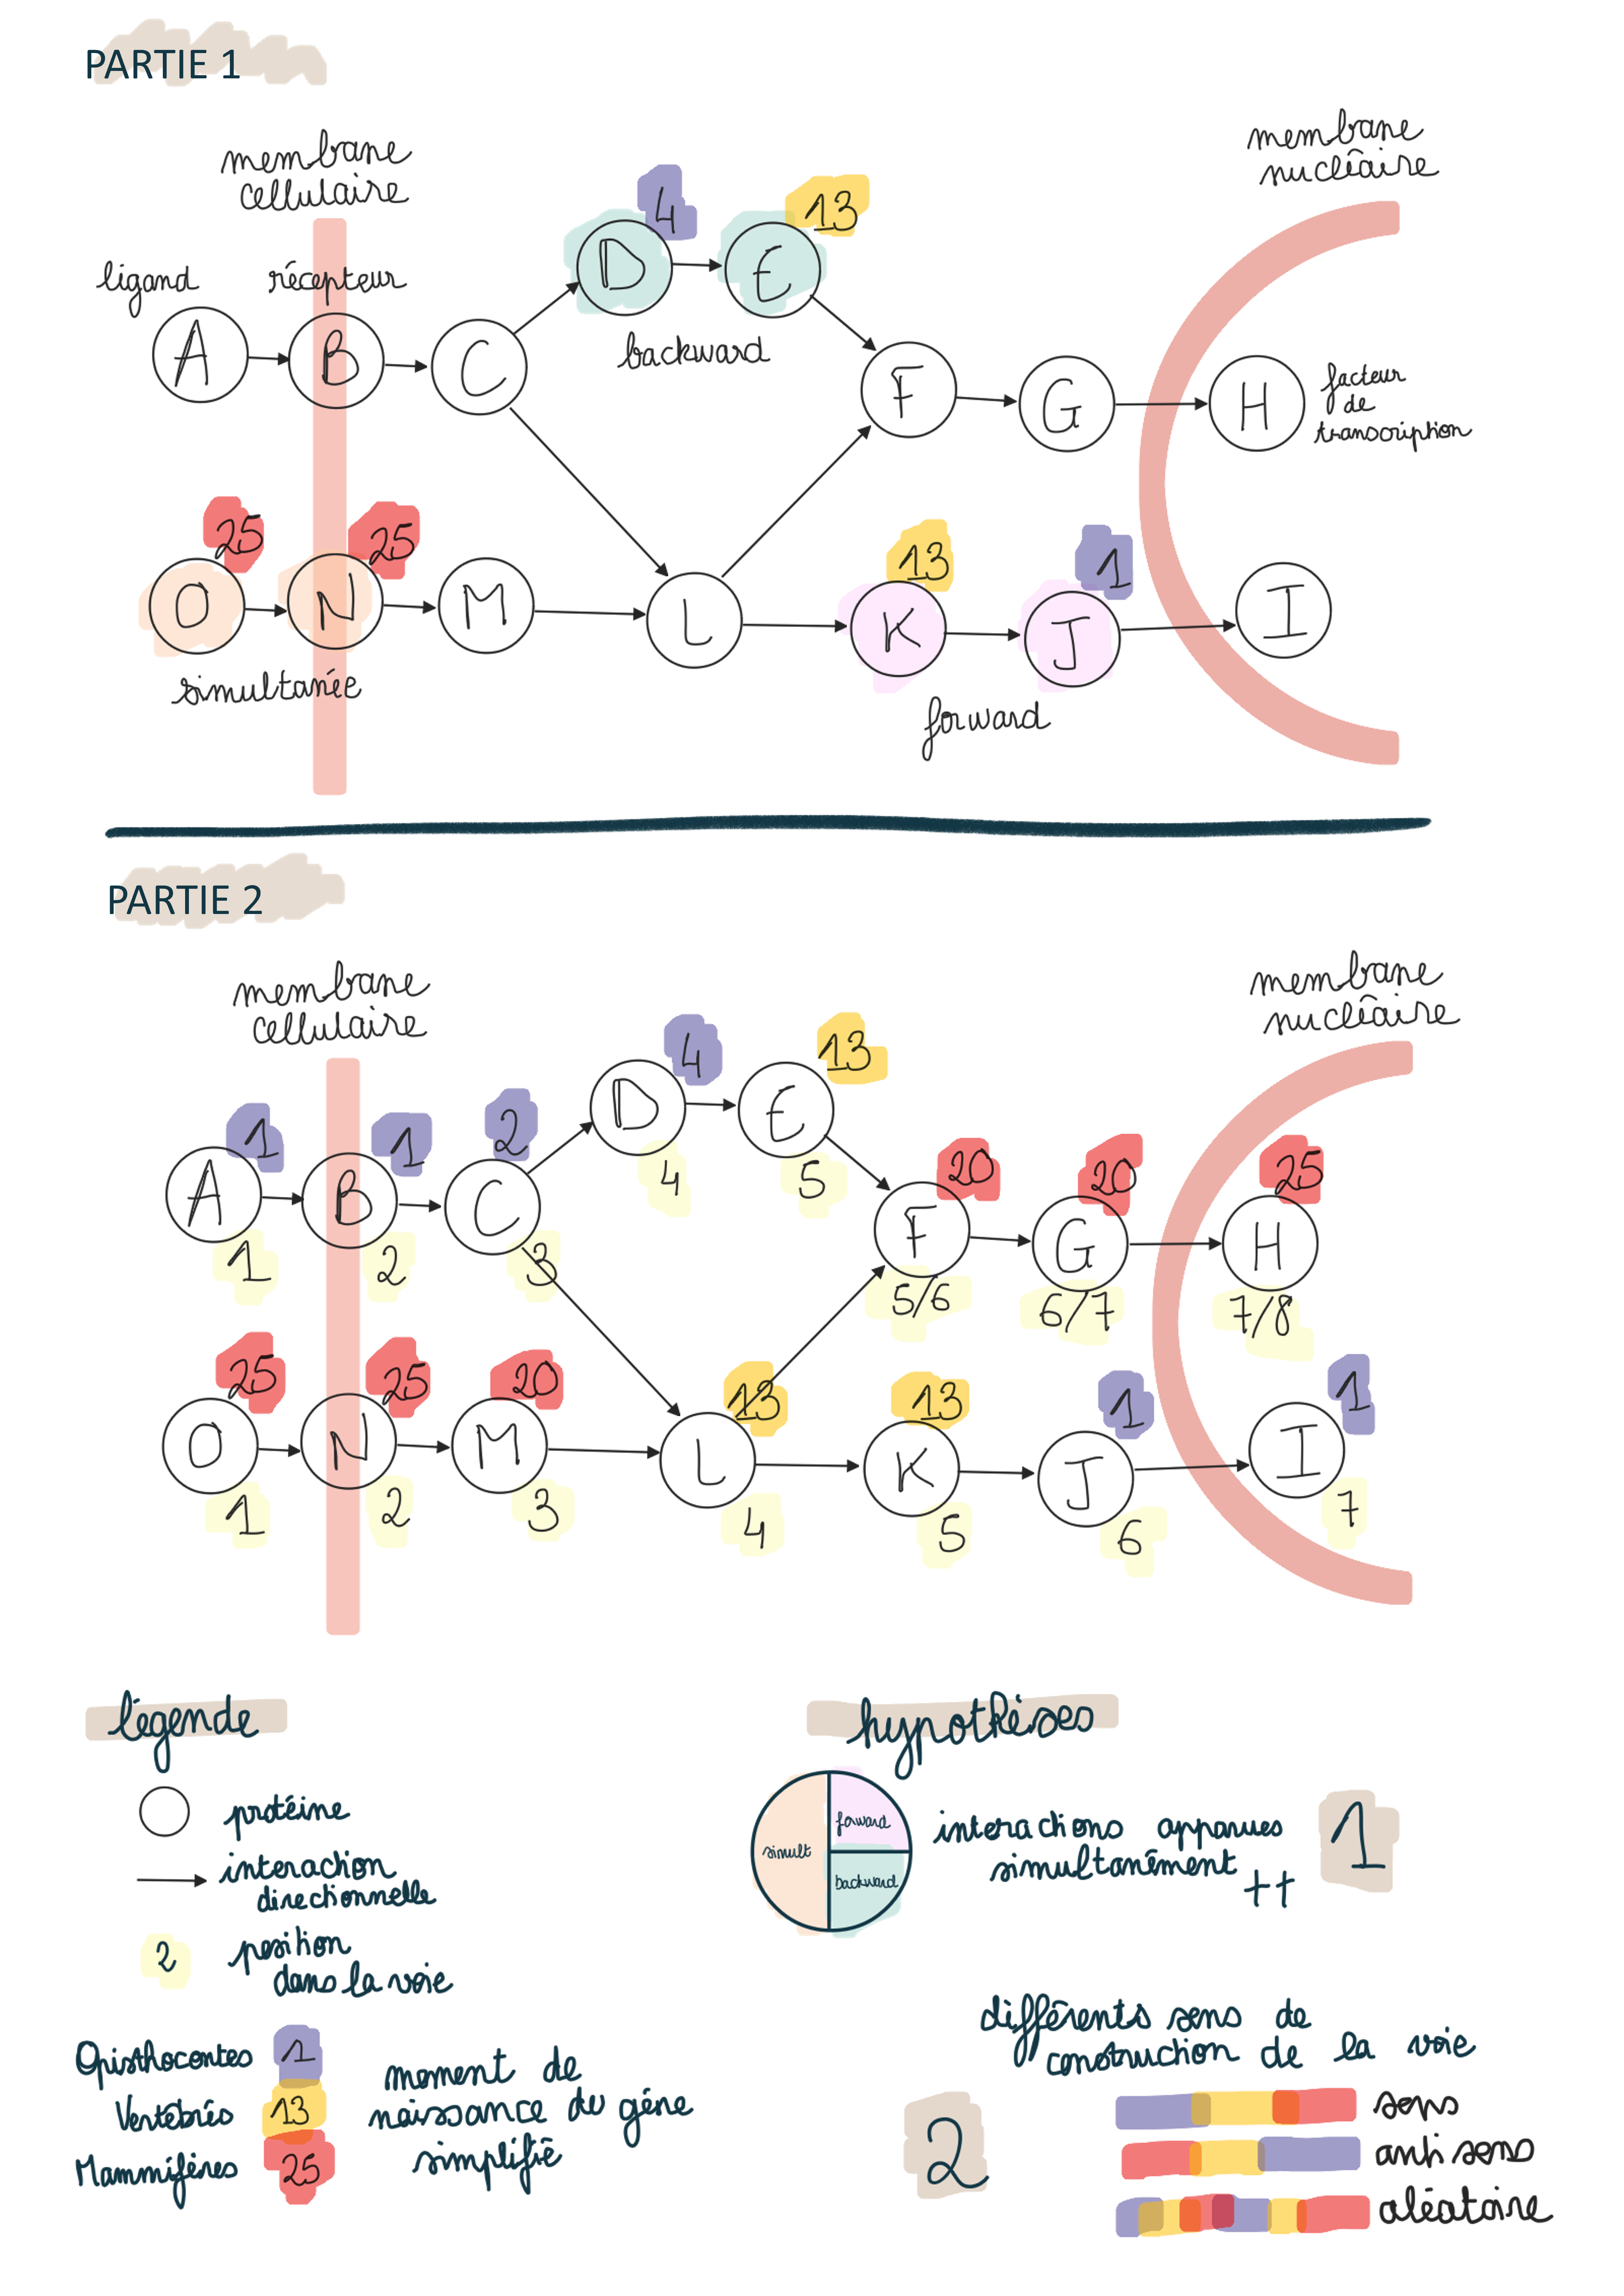
\includegraphics[width=1\textwidth]{figures/corps/figure14.png}
    \caption{Schéma récapitulatif de l'étude 1}
    \label{fig:14_schéma1}
\end{figure}

\section{Article}\label{art1}
\includepdf[scale=0.9,pages=1-23,pagecommand={\thispagestyle{plain}}]{figures/articles/article1.pdf}

\includepdf[scale=0.80,pages=1-11, nup=1x2,pagecommand={\thispagestyle{plain}}]{figures/articles/figures-article1.pdf}

    \chapter{Article 2 - Moment d’apparition des gènes impliqués dans une voie de transduction du signal humaine}
\thispagestyle{firstpage}
\onehalfspacing

\section{Contexte de l'étude}
\par Un des piliers majeurs de l’évolution est la naissance de nouveaux gènes, et elle est en partie due aux duplications de gènes et de génomes. Deux duplications de génomes complets (WGD) sont survenues à la racine des vertébrés lors de la scission avec les invertébrés. De plus, le clade des téléostéens a subi une 3$\textsuperscript{ème}$ duplication de génome complet, et une partie de ces espèces (les salmonidés et les carpes) une 4$\textsuperscript{ème}$. Les périodes de duplications de génome sont suivies de pertes massives de gènes dupliqués. Le clade des téléostéens est donc un modèle de choix pour étudier la capacité de ces gènes à rester à l’état de gènes dupliqués ou leur retour sous forme de singleton. Cette étude est présentée sous forme de schéma récapitulatif en Figure ~\ref{fig:15_schéma2} page ~\pageref{fig:15_schéma2} et est suivie d’un article (page \pageref{art2}) publié dans le journal Heliyon : \parencite{picolo_genes_2021}.

\section{Matériels et méthode}
\par Pour cette étude, nous avons récupéré un ensemble de 2 298 gènes uniques impliqués dans 47 voies de signalisation humaine dans la base de données KEGG V104. Les voies et leurs caractéristiques sont présentées dans le Tableau \ref{table:voiecaracteristiq}.  
\par Afin de déterminer la quantité d’orthologues téléostéens pour chacun de nos gènes impliqués dans une voie de signalisation, nous avons récupéré l’ensemble des orthologues téléostéens par la plateforme Biomart d’Ensembl V107. L’ensemble des espèces de téléostéens dont le génome annoté est disponible sur Ensembl a été utilisé, soit 63 espèces, dont 54 espèces ayant subi 3 duplications de génome complet, et 9 ayant subi 4 duplications de génome complet. Nous avons conservé 2 groupes distincts pour l’ensemble de l’étude : les 3 WGD, et 4 WGD. Nous avons récupéré toutes les interactions gène-gène pour regarder la quantité de paralogues en interaction (que nous appellerons « stœchiométries ») dites :
\begin{itemize}
    \item respectées avec n :n,
    \item non respectées avec n :m dont m>n, 
    \item ou perdues totalement ou partiellement avec 0 :n,
\end{itemize}
et si une pression subsiste dans la relation pour maintenir les partenaires en quantité égale au sein des espèces, mais également au sein des interactions. La proportion des gènes impliqués dans une voie de signalisation dans les différentes stœchiométries sera statistiquement comparée, à l’ensemble des gènes des génomes (Chi2 et test hypergéométrique). 

\section{Résultats}
\par Dans un premier temps, nous avons constaté que pour toutes les espèces 3 WGD, nous avons plus souvent retrouvé nos gènes sous la forme dupliquée que les gènes du génome (p-value < 0,001) et pour toutes les espèces 4 WGD, nous avons plus souvent retrouvé nos gènes sous forme triplicat ou plus que les gènes du génome (p-value < 0,00002). Concernant les quantités de gènes pour les interactions gène-gène, nous retrouvons une majorité d’interactions à stœchiométrie 1 :1 (30,3\%) pour les espèces 3 WGD, puis les interactions 1 :2 à 27,3\% en moyenne et enfin la stœchiométrie 0 :1 à 18\% qui représentent une perte partielle de l’interaction chez les téléostéens. Tandis que pour les espèces 4 WGD, on constate une majorité d’interactions 2 :2 (15,8\%), puis les interactions 2 :4, à 14\% en moyenne et enfin les interactions 0 :2, à 11,6\%. Pour les deux groupes étudiés (3 et 4 WGD), nous observons une quantité d’interactions partiellement ou totalement perdues importante (0 :0, 0 :1, 0 :2, 0 :3, 0 :4 allant de 0,1\% à 22.1\% en fonction des espèces). Les stœchiométries non respectées sont majoritaires dans l’ensemble des voies de signalisation allant de 34\% à 70\%. Mais 2 voies se démarquent avec une majorité d’interactions n :n (Hedgehog à 65\% et Estrogen à 50\%). De plus, aucune interaction n’est totalement perdue pour 3 voies de signalisation chez les téléostéens : JAK-STAT, FoxO et Glucagon. 

\section{Conclusion}
\par Nos résultats montrent que les gènes des voies de signalisation restent plus souvent en duplicat ou en triplicat chez les espèces 3 ou 4 WGD de téléostéens que les gènes du génome. Nous retrouvons une majorité d’interactions gène-gène à stœchiométrie respectée en moyenne chez les téléostéens (1 :1 et 2 :2 respectivement pour les 3 et 4 WGD). Cependant, les stœchiométries restent nettement différentes et en fonction de la voie étudiée. Il faut toutefois noter l’exception d’une absence de perte totale pour les 3 voies JAK-STAT, FoxO et Glucagon. 

\begin{figure}[H]
    \centering
    \includegraphics[width=1\textwidth]{figures/corps/figure15.png}
    \caption{Schéma récapitulatif de l'étude 2}
    \label{fig:15_schéma2}
\end{figure} 
\newpage

\section{Article}\label{art2}
\setlength{\headheight}{17.30428pt}
\addtolength{\topmargin}{-5.30428pt}
\includepdf[scale=0.9,pages=1-8,pagecommand={\thispagestyle{plain}}]{figures/articles/pico-2021.pdf}
    \chapter[Discussion]{Discussion}
\thispagestyle{firstpage}
\onehalfspacing

\section{Étude sur les moments d’apparition}
\par Dans un premier temps, notre étude a permis de mettre en lumière trois scénarios possibles sur la construction d’une voie de signalisation intracellulaire humaine. Notre premier scénario était que les voies sont arrivées dans le sens amont vers aval, donc des ligand-récepteur aux facteurs de transcription. Cette hypothèse nous semblait être la moins probable au vu des résultats de l’étude d’Anna Grandchamp durant sa thèse \parencite{grandchamp_synchronous_2018}. En effet, ce travail a montré que 38\% des récepteurs sont apparus avant leur ligand contre 21\%, apparus après leur ligand. Or dans notre cas, le ligand est à la position 1 dans la cascade de signalisation, et le récepteur à la position 2 ce qui favoriserait la deuxième hypothèse. Cependant, nous avons travaillé sur un plus grand nombre d’espèces : 315 au lieu des 145 espèces dans l’étude précédente, et sur 25 clades au lieu de 10. Cette augmentation des données permet probablement d’être plus précis dans la recherche d’orthologues dans l’arbre de la vie, et d’être plus résolutifs concernant les nœuds d’apparition. Ce scénario pourrait expliquer 10 des voies KEGG. 
\par Notre deuxième scénario concerne les voies qui se sont construites de l’aval vers l’amont, donc des facteurs de transcription vers les ligand-récepteur et a été validé pour 25 voies de notre étude (r < 0, p-value < 0.02) dont 3 voies (Adipocytokine, Fc epsilon RI et VEGF) pour lesquelles la corrélation est particulièrement forte (r > 0.5, p-value < 3.15E-8). Ce scénario peut également être motivé par d’autres éléments, comme le fait que les protéines en aval de voie de signalisation sont connectées avec plus de partenaires que les protéines en amont de la voie. La “multi-connectivité“ d’une protéine augmente ses contraintes évolutives car cela imposerait une coévolution à ses différents partenaires \parencite{fraser_evolutionary_2002, hahn_molecular_2004, krylov_gene_2003}. 
\par Pour autant, cela pourrait également venir des types de fonction en amont des voies et en aval qui peuvent être différents. En effet, dans l’étude d’\cite{alvarez-ponce_relationship_2012}, il est montré une différence notable entre la nature des protéines en début et en fin de voie. Les protéines en amont d’une voie sont logiquement enrichies en activité kinases (q = 2,24 × 10 –4, q étant la p-value corrigée par Benjamini et Hochberg) tandis que les protéines en aval sont enrichies en activités de transporteur transmembranaire ionique (q = 2,65 × 10 –5 ). De notre côté, nous n’avons pas regardé la \textit{Gene Ontology} de nos protéines en début et en fin de voie, mais cela pourrait être reconsidéré.
\par Et notre dernier scénario concernait une absence d’ordre pour la construction d’une voie de signalisation. Ce scénario semble concerner 12 voies de notre étude. 
\par Par ailleurs, l’étude d’Alvarez-Ponce qui comprenait 1 049 protéines et 2 436 interactions, a montré qu’il n’y avait pas d’incidence entre la position hiérarchique d’une protéine dans une voie et leur taux d’évolution. La particularité de l’étude était qu’il partait sans a priori de la voie c’est-à-dire qu’ils ont utilisés uniquement des interactions et non pas des voies définies comme le fait KEGG et la position hiérarchique était déterminée en fonction de leur position dans la voie (\textit{upstream} ou \textit{downstream}). Le taux d’évolution représente le ratio entre les mutations silencieuses et les mutations faux sens pour des séquences hommes \textit{vs.} souris \parencite{alvarez-ponce_relationship_2012}. Dans notre cas, le taux d’évolution (dN/dS) n’a pas été calculé. Nous pourrions également envisager de le faire pour notre étude.
\par Le taux d’évolution est donc différent du moment d’apparition, mais peut lui être lié. Plus un gène a un taux d’évolution élevé, par exemple s’il est soumis à une sélection positive, et plus il y a de chance qu’il ait beaucoup divergé jusqu’à devenir une sorte de nouveau gène et donc de ne pas être détecté en tant qu’orthologue. Dans ce cas, le moment d’apparition du gène humain pourrait d’être plus éloigné que pour un gène présentant une vitesse d’évolution plus lente. 
\par Nous avons fait le choix durant cette étude de partir de l’homme, qui est l’espèce la plus référencée, et de partir d’un échantillon de voies de signalisation décrite comme telle sur la base de données KEGG. 
\par De plus, nous avons imaginé 3 scénarios possibles, mais il existe d’autres scénarios que nous n'avons pas exploré. On peut évoquer maintenant que des voies pourraient être construites à partir d’une chaîne d’interactions protéiques ancestrales « simple » et se serait vu complexifiée à travers l’évolution et les différentes spécificités des espèces. Cette réflexion s’est notamment faite en analysant de plus près la sous-voie RTK/RAS/ERK qui est présente dans 22 voies sur 47 de notre étude. Les éléments de cette sous-voie sont apparus tôt dans l’arbre de la vie puisque la voie est commune aux drosophiles, aux vers et aux humains \parencite{ashton-beaucage_signalisation_2010}. 
\par Cette première étude a également mis en lumière deux nœuds qui semblent être des pivots de l’évolution pour les gènes de voie de signalisation : le nœud des Opisthocontes, et celui des Vertébrés. Ce sont ces mêmes nœuds qu’Anna Grandchamp avait mis en évidence dans son étude sur les ligand-récepteur \parencite{grandchamp_synchronous_2018}. Le nœud des Opisthocontes est un nœud peu surprenant au vu de la littérature. On constate que la comparaison levures-mammifères a montré de grandes similitudes de structure de réseaux moléculaires \parencite{cross_evolution_2011}. Concernant le deuxième nœud évolutif notable, le nœud des Vertébrés, il vient prendre son origine après deux duplications de génome, et il a été montré également que les gènes issus de duplication de génome avaient une évolution lente comparée aux gènes dupliqués à petite échelle \parencite{satake_evolution_2012}. Dans cette même étude également, sont pointés du doigt les gènes d’expression ubiquiste qui évolueraient moins vite que les gènes d’expression tissulaires spécifiques. Et c’est effectivement un point qui pose une autre question : Est-ce que les gènes impliqués dans des voies de signalisation activées dans la majorité des cellules évoluent moins vites que des voies spécifiques de tissus ? Effectivement, certaines voies sont essentielles à toutes les cellules, notamment les voies menant à la croissance cellulaire ou la division cellulaire comme la voie cAMP \parencite{sassone-corsi_cyclic_2012} et d’autres spécifiques à une fonction comme les voies de l’immunité ou la voie Hippo régulatrice de la contraction musculaire entre autres grâce à sa capacité régulatrice de la taille des cellules \parencite{zhao_hippo_2011}. 
\par Un début de réponse peut être donné concernant les gènes des voies de l’immunité puisque nous avons trouvé que 72\% des gènes des voies de l’immunité sont apparus après le nœud des Vertébrés. Ce constat rejoint par ailleurs la littérature qui évoque l’évolution rapide de ces gènes \parencite{cooper_evolution_2006, schlesinger_coevolutionary_2014}. 
\par Il aurait été intéressant de confronter différentes voies de signalisation présentes chez des espèces différentes de l’arbre de la vie des Opisthocontes. Seulement, la voie MAPK est l’unique voie disponible chez la levure sur KEGG.
\par Il faut tout de même émettre des réserves sur nos résultats car un moment d’apparition pour une interaction ne signifie pas qu’elle est fonctionnelle. Tout comme un moment d’apparition d’un gène ne rend pas la protéine fonctionnelle chez toutes les espèces concernées. Il faudrait, pour confirmer ces résultats, valider fonctionnellement les interactions chez les espèces avec l’ancêtre commun le plus éloigné de l’homme par un système de double hybride par exemple. Un système de double hybride permettrait de valider une interaction entre deux protéines, mais dans des conditions artéfactuelles, pouvant être très éloignée de la réalité. Ce qui serait un travail colossal et très coûteux pour le nombre d’interactions et le nombre d’espèces différentes. On pourrait également utiliser des techniques novatrices et relativement inexplorées comme la résurrection des gènes. Des travaux ont été entamés sur la résurrection de protéines afin de mieux connaître les fonctions des gènes ancestraux. La technique consiste à réintégrer dans un organisme un gène jusqu’alors inactif ou désactivé chez cette espèce par le biais d’un système tel que Crispr-Cas9. Bien que ce soit une technique complexe, elle se veut prometteuse \parencite{harms_evolutionary_2013}. Une autre façon de répondre à ces questions serait de modéliser les structures tridimensionnelles des protéines ancestrales. La technologie AlphaFold2 est une avancée majeure dans le domaine de la prédiction de la structure des protéines \parencite{cramer_alphafold2_2021}. Avec cet outil, nous pourrions pousser l’étude d’un point de vue tridimensionnel et se demander pour chacune des protéines des voies de signalisation, et à travers l’arbre de la vie, à quel moment ont eu lieu les modifications tridimensionnelles, si changement il y a. Et pourquoi ne pas rêver d'arbres phylogénétiques de gènes basés non pas sur des homologies de séquences primaires, mais sur des homologies de structure 3D des protéines ?
\par Les gènes et leur évolution sont des sujets qui animent la communauté scientifique. Par ailleurs, l’évolution est constante et perpétuelle, ce qui mène à des questionnements peut être plus hardis. Par exemple, on pourrait se poser la question de futures duplications de génome chez certains clades. Certaines espèces vivant dans des régions arides ont peut-être déjà doublé certains de leurs gènes pour mieux supporter la chaleur. Et si les températures continuent d'augmenter, il est possible que, sur plusieurs siècles, les poissons développent des duplications génétiques pour accroître leur résistance à la chaleur. De même, ils pourraient évoluer pour mieux s'adapter à des environnements plus salins si les rivières venaient à s'assécher complètement. Grâce au système de Crispr-Cas9, nous arrivons de mieux en mieux à modifier les génomes précisément. Il pourrait donc être envisageable de dupliquer des génomes. Mais ceci reste encore très utopique. 
\par Dans un registre beaucoup plus réalisable, il serait intéressant de regarder plus en profondeur les gènes orphelins, car l’étude a montré qu’une majorité des protéines en interactions attendaient leur partenaire (84\% d’interactions asynchrones). Que font les protéines sans leur partenaire ? Premièrement, nous avons choisi de centrer notre étude sur les gènes des voies de signalisation qui représentent 3 000 interactions protéine-protéine unique, ce qui en fait un petit échantillon sur les 93 000 interactions protéine-protéine uniques recensées par \cite{luck_proteome-scale_2017}. Et deuxièmement, des études ont été menées sur des récepteurs nucléaires orphelins, mais les résultats sont trop divergents, ce qui montre bien la difficulté de la problématique \parencite{markov_origin_2011}. 

\newpage
\section{Étude sur les téléostéens}
\par Dans un deuxième temps, nous avons étudié la stœchiométrie des interactions chez les espèces 3 WGD et 4 WGD du clade des téléostéens. Cette étude a montré que pour l’ensemble des espèces de poissons téléostéens, la stœchiométrie des interactions était respectée en fonction du nombre de duplications de génome des espèces. Pour autant, une notion n’a pas été prise en compte : les paralogues retrouvés sont-ils des paralogues ohnologues, ou des paralogues « simples ». On recense environ 26\% de gènes ohnologues chez le poisson zèbre \parencite{howe_zebrafish_2013} et environ 44\% de gènes ohnologues chez les salmonidés \parencite{dimos_homology_2023}.
\par Ce que nous avons trouvé étonnant, ce sont les résultats concernant les espèces 4 WGD. Pour rappel, les clades des salmonidés et des carpes ont vécu indépendamment une 4$\textsuperscript{ème}$ duplication de génome, à des temps différents et pour autant, les résultats concernant les différentes stœchiométries possibles pour ces deux groupes d’espèces étaient sensiblement les mêmes. La 4$\textsuperscript{ème}$ duplication de génome des salmonidés a eu lieu, il y a environ 80 millions d’années \parencite{lien_atlantic_2016}, tandis que celle des carpes a eu lieu il y a environ 14 millions d’années \parencite{jaillon_genome_2004, kon_single-cell_2022, xu_allotetraploid_2019}. Nous avons constaté des proportions similaires concernant les différentes stœchiométries, mais nous n’avons pas étudié si les interactions en question étaient les mêmes pour les deux clades indépendants. Nous pourrions lister ces interactions afin de mieux comprendre si la pression de maintien des interactions en stœchiométrie respectées étaient les mêmes malgré une divergence aussi lointaine. 
\par De plus, il serait intéressant d’avoir une approche par voie pour les téléostéens, c’est-à-dire regarder si des sous-voies au sein des voies sont en stœchiométrie respectée. Dans notre cas, nous avons étudié interaction par interaction et non directement en utilisant la voie. C’était dû à un manque de maîtrise des outils igraph au moment de l’étude, mais ça pourrait mettre en lumière une pression de maintien en duplicat ou même de retour en singleton par la voie au sein des téléostéens. Ça pourrait donner également des indications sur les voies de signalisation existantes chez les téléostéens qui sont encore assez peu étudiées. 
\par Nous avons également noté une part non négligeable de gènes absents chez les téléostéens. Les interactions partiellement ou totalement perdues chez les téléostéens étaient en moyenne à hauteur de 25\%. Dans quelques cas, notamment dans le cas où nous avions une perte chez quelques espèces tandis que l’interaction était présente chez le reste des espèces, nous avons retrouvé des traces de pseudogènes. Mais, dans le cas où nous ne retrouvions pas l’interaction pour l’ensemble du clade, nous avons émis l’hypothèse que les gènes et donc les interactions seraient nées après. Seulement, il serait pertinent de croiser nos deux études et de regarder si les gènes étaient apparus avant le clade des Vertébrés, mais se seraient éteints chez les téléostéens car non essentiel aux espèces. De plus, cette hypothèse est un biais de notre étude que nous pourrions améliorer en redéfinissant les conditions d’admission d’un nœud d’apparition. Nous pourrions convenir qu’il faut plus de 80\% (par exemple) de présence du gène dans l’ensemble des espèces entre l’homme et le nœud le plus éloigné où on retrouve un orthologue.  


\newpage
\section{Limite du matériel et de la méthode}
\par Durant ces différentes études, nous avons fait des choix de matériel à utiliser et d’une méthodologie à suivre. Nous avons longuement hésité entre une étude exhaustive avec toutes les voies de signalisation que proposait KEGG, et même pousser l’exhaustivité et regrouper des données de différentes bases de données comme celles de la base de données BioGrid, String, Reactome ou encore NetPath qui sont également des bases de données d’interactions protéiques, ou faire une étude plus spécifique sur une voie de signalisation précise qui pourrait notamment intéresser l’équipe de recherche dans laquelle j’ai réalisé ma thèse. Nous avons fini par trancher sur une liste de 47 voies de signalisation sur la base de données KEGG, car c’était la mieux référencée \parencite{rigden_26th_2019}. 
\par Concernant l’arbre et les espèces utilisées, Anna Grandchamp avait utilisé ces deux mêmes bases de données. Cette thèse s’inscrivant naturellement à la suite de celle d’Anna Grandchamp en 2018, il y avait un souhait de confronter nos résultats aux siens et donc d’utiliser les mêmes outils. Pour autant, la base de données Ensembl et par extension Genomicus a connu un changement important entre la version 93 (janvier 2018) et la version 94 (juillet 2018). En version 93, les arbres étaient présentés de telle façon à ce que l’ensemble des paralogues et orthologues d’un gène soient présents dans un arbre unique. Seulement, avec les ajouts de nouvelles espèces séquencées, la base de données a changé de méthodes de clustering des gènes et de nombreux liens de paralogie ont disparu, rendant impossible la visualisation des grandes familles de gènes. Les arbres ont donc été redécoupés en sous-arbres \parencite{emily_changes_2018}. De ces changements majeurs, nous nous sommes longuement posé la question de savoir si nous devions rester sur les arbres de version 93, ou si nous prenions les versions les plus récentes. Pour nos questions de recherche, nous avons décidé de prendre les plus récentes versions afin d’avoir le plus d’espèces possibles et de recouvrir au maximum l’arbre de la vie des Opisthocontes et plus précisément des téléostéens pour l’étude 2. 
\par Et afin de valider un moment d’apparition, il pourrait être réalisable de faire des BLAST pour chacun des gènes avec l’espèce ancestrale la plus éloignée d’un point de vue évolutif. 
\par De plus, nous avons été confrontés à de nombreux questionnements concernant la gestion des données KEGG. En effet, KEGG reste une base de données renseignée à la main, et par facilité de compréhension, des voies peuvent afficher une famille de gènes paralogues derrière une étiquette portant un nom plus générique. Seulement, elle ne le fait pas systématiquement et des familles de gènes peuvent se retrouver dans des étiquettes uniques, comme c’est le cas par exemple pour la voie PPAR, les gènes PPAR alpha, beta/delta et gamma sont des paralogues qui sont affichés distinctement dans la voie. L’hypothèse émise était que les paralogues ont des fonctions différentes et des interactions spécifiques comme des interactions communes entre elles, comme semble le montrer la voie. Pour autant, il a fallu décider de ce que l’on faisait dans des cas comme PPAR. Nous nous sommes également demandé s’il n’était pas préférable de gérer tous les paralogues de la même façon et de prendre le même ancêtre commun pour une même famille de gènes. Là encore, nous avons discuté pour savoir quel ancêtre commun nous prenions si les arbres des différents paralogues n’étaient pas d’accord. Prenions-nous le plus ancien, le plus récent, le plus représenté ? Nous avons fini par faire l’étude avec toutes les configurations possibles avant de trancher sur celle qui nous semblait présenter le moins de biais : la gestion des paralogues telle que présenté par KEGG, soit en groupe, soit unique. Et pour les gènes avec de nombreux paralogues en groupe, de prendre le nœud ancestral le plus éloigné. 
\par Par souci de simplification des voies, nous avons également omis l’information de l’interaction, à savoir si l’interaction était activatrice, ou inhibitrice, ou autre. Cependant, il faudrait confronter nos résultats à cette dimension-là. Nous pourrions séparer les interactions en fonction de leur type et regarder si des corrélations se dégagent. 

\newpage
\section{Perspectives}
\par Les résultats que nous avons obtenus concernant le moment d’apparition des gènes peuvent faire l’objet de projets complémentaires. J’aimerais ajuster plus précisément les moments d’apparition en regardant chez les clades plus éloignés encore comme celui des plantes par exemple ou celui des bactéries. Le génome de l’homme comportant environ 25\% de ses gènes en commun avec les plantes, il est fort possible qu’un certain nombre de gènes soient des gènes de voie de signalisation.
\par Par ailleurs, nous aimerions proposer à la base de données KEGG d’implémenter un nouvel outil faisant apparaître les moments d’apparitions des gènes directement sur les voies avec un système de couleur comme nous l’avons réalisé. En poussant nos idées, nous pourrions également afficher le nombre d’orthologues retrouvés pour une espèce donnée, cela permettrait en un coup d’œil de connaître la présence ou non d’un gène chez une espèce, et de connaître la stœchiométrie de ces interactions dans un cadre de voie de signalisation. 
\par Nos résultats concernant la coévolution de gènes impliqués en interactions nous ont donnés envie de regarder ce qu’il en était concernant les gènes pro-apoptotiques et anti-apoptotiques. En effet, il serait intéressant de regarder qui de l’un ou de l’autre apparaît le premier. Cela rejoindrait les études précédentes sur les ligand-récepteur, et les gènes des voies de signalisation. 
\par Bien évidemment, il serait plus juste scientifiquement de valider tous nos résultats avec des approches de biologie expérimentale. Cependant je n’ai pas les outils pour imaginer des expériences poussées, et de plus, en travaillant sur un si large matériel comme nous l’avons fait ici, il faudrait faire des choix. 

    \chapter{Conclusion}
\thispagestyle{firstpage}
\onehalfspacing

\par Nos travaux ont testé trois scénarios possibles de construction des voies de signalisation. Nous mettons également en lumière deux moments d’apparition clés dans l’arbre de la vie pour les gènes impliqués dans une voie de signalisation qui sont le nœud des Opisthoconte et celui des Vertébrés. Au regard de ces résultats, la double duplication de génomes à l’émergence des Vertébrés peut être à l’origine de la naissance de nouveaux gènes de voie de signalisation. Nous avons poussé nos recherches en détail pour connaître le comportement des interactions chez des clades les plus anciens des vertébrés, à savoir les téléostéens qui ont subi 3 ou 4 duplications de génome. Nous avons constaté que les orthologues téléostéens des gènes humains des voies de signalisation restaient plus souvent en duplicat ou en triplicat chez les espèces 3 ou 4 WGD téléostéens que les gènes du génome. Et nous avons retrouvé une majorité d’interactions protéine-protéine à stœchiométrie respectée en moyenne chez les téléostéens.
    \chapter[Annexes]{Annexes}
\thispagestyle{firstpage}

\minitoc
\newpage

\section{Article 3}\label{article3}
\includepdf[scale=0.85,pages=1-6,pagecommand={\thispagestyle{normalpage}}]{figures/articles/pico-2023.pdf}

\section{Article 1 - Suppl. Data 1}
\textbf{Suppl. Data 1 - Distribution of deltas of node of birth of genes encoding proteins involved in all the pathways, according to the node of birth of each gene}\\
Legend: Deltas are calculated via clade of birth rank for the A gene - clade of birth rank for the B gene for the interaction A $\rightarrow$ B. For example, if gene A was born at the blue clade (clade 1), and the clade of birth of B is 11, the A $\rightarrow$ B delta is -10. Moreover, in this case, it is a backward relationship, because A was born before B.
\par The pathways are in the following order:
PPAR, MAPK, ErbB, Ras, Rap1, Calcium, cGMP-PKG, cAMP, Chemokine, NF-kappa B, HIF-1, FoxO, Sphingolipid, Phospholipase D, p53,  mTOR, PI3K-Akt, AMPK, Wnt, Notch, Hedgehog, TGF-beta, VEGF, Apelin, Hippo, Toll-like receptor, NOD-like receptor, RIG-I-like receptor, C-type lectin receptor, JAK-STAT, IL-17, T cell receptor, B cell receptor, Fc epsilon RI, TNF, Neurotrophin, Insulin, GnRH, Ovarian steroidogenesis, Estrogen, Prolactin, Thyroid hormone, Adipocytokine, Oxytocin, Glucagon, Relaxin, AGE-RAGE.

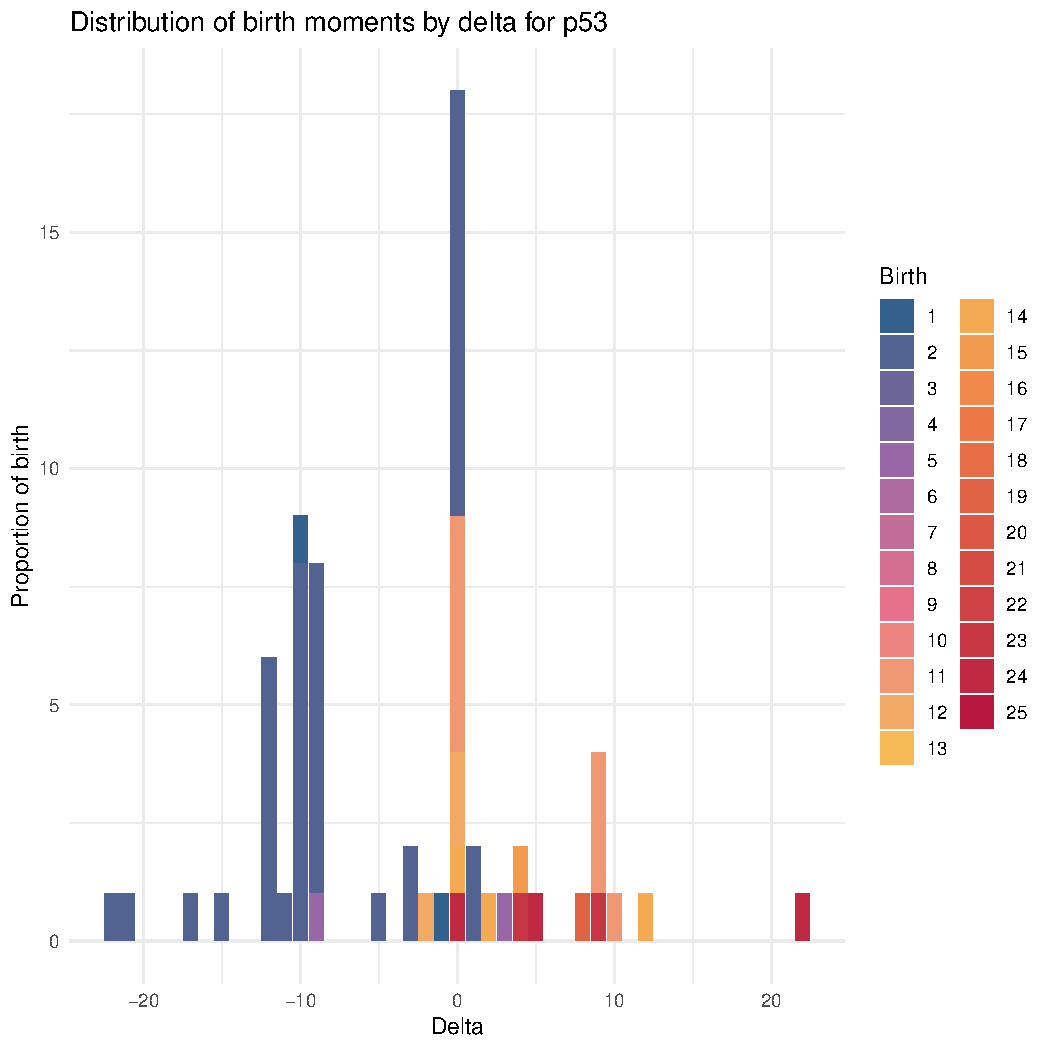
\includepdf[scale=0.85,pages=1-47, nup=1x2, pagecommand={\thispagestyle{normalpage}}]{figures/suppldata/suppldata1.pdf}

\section{Article 1 - Suppl. Data 2}
\textbf{Suppl. Data 2 - Colored KEGG pathways depending on the node of birth of each protein}\\
Legend: Each color represents a clade. The white rectangles correspond to the genes for which we have not been able to determine the node of birth due to lack of information about the gene. The KEGG legend is available here: \href{https://www.genome.jp/kegg/document/help_pathway.html}{https://www.genome.jp/kegg/document/help}
\par The pathways are in the following order:
PPAR, MAPK, ErbB, Ras, Rap1, Calcium, cGMP-PKG, cAMP, Chemokine, NF-kappa B, HIF-1, FoxO, Sphingolipid, Phospholipase D, p53,  mTOR, PI3K-Akt, AMPK, Wnt, Notch, Hedgehog, TGF-beta, VEGF, Apelin, Hippo, Toll-like receptor, NOD-like receptor, RIG-I-like receptor, C-type lectin receptor, JAK-STAT, IL-17, T cell receptor, B cell receptor, Fc epsilon RI, TNF, Neurotrophin, Insulin, GnRH, Ovarian steroidogenesis, Estrogen, Prolactin, Thyroid hormone, Adipocytokine, Oxytocin, Glucagon, Relaxin, AGE-RAGE.

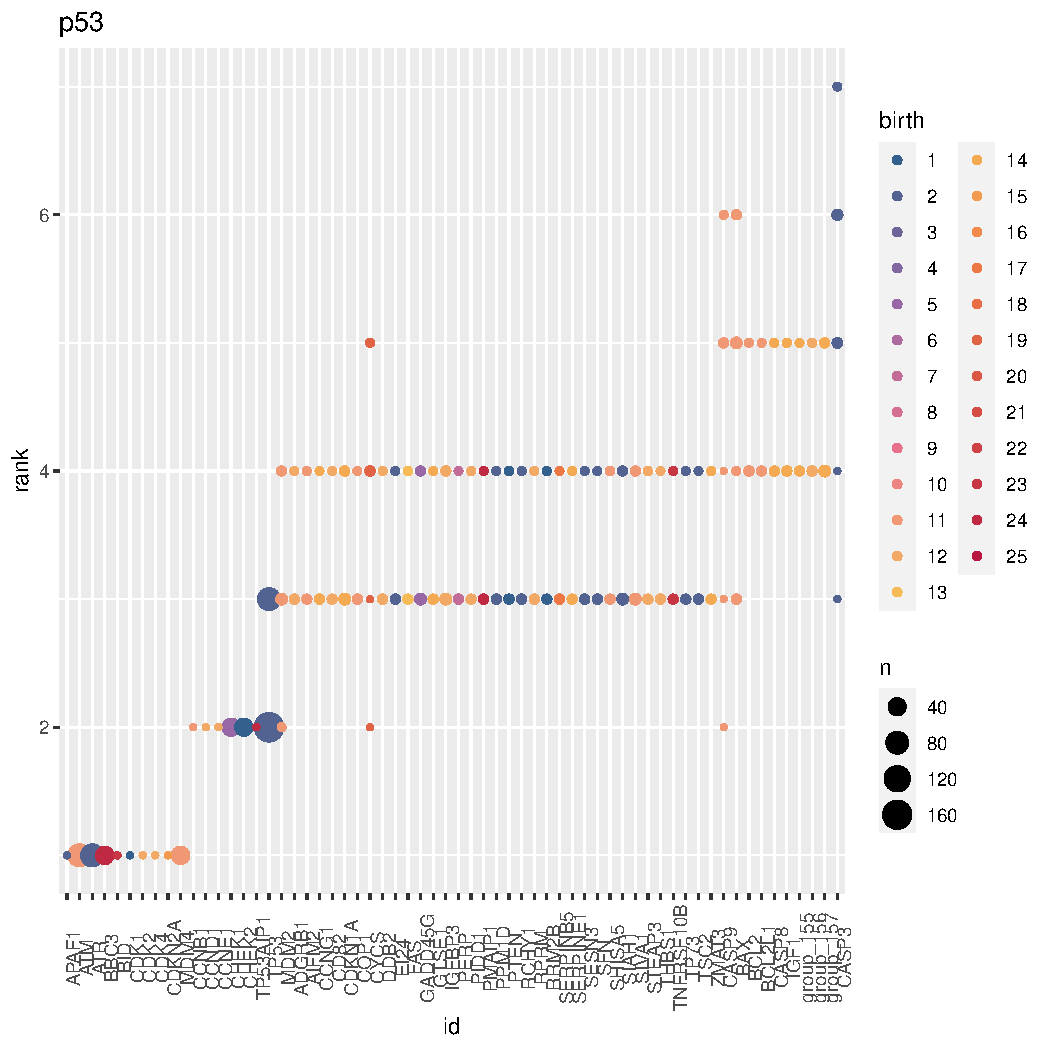
\includepdf[scale=0.85,pages=1-47, nup=1x2, pagecommand={\thispagestyle{normalpage}}]{figures/suppldata/suppldata2.pdf}

\section{Article 1 - Suppl. Data 3}
\textbf{Suppl. Data 3 - Animal tree of life and clades of study}\\
Legend: Tree of life of the 315 species studied here, generated using the information available in Ensembl and Ensembl Metazoa, and with R's ape package \parencite{paradis_ape_2019}. The tree is rooted to reflect the phylogeny of the \textit{Opisthokonta}, and the branches are not to scale. The colors are those used in the figures of the article. Each clade is represented by one or more species in our database.

\includepdf[scale=1, pagecommand={\thispagestyle{normalpage}}]{figures/suppldata/suppldata3.pdf}


    
    
    \printbibliography
        
    \pagededos
\end{document}
